\chapter{Architectural aspects of the system}\label{ch:architectural-aspects-of-the-system}


\section{Application architecture and related comments}\label{sec:application-architecture-and-related-comments}
As a programmers, I believe all we have faced the cases of crucial over-engineering during the implementation of some
software product.
For the programmer, it is a vital point to follow two separated, but closely related software development principles,
such that KISS [\cite{alwin2016kiss}], and YAGNI [\cite{da2018evolution}].
As the main topic of our thesis is to implement Instant Messaging System following the security and privacy aspects.
We consider to following above-mentioned development principles KISS and YAGNI and approach
a well-known N-tier application Monolithic architecture [\cite{bucchiarone2018monolithic}], which provides a model by which developers can
create flexible and reusable applications.
By segregating an application into tiers, developers acquire the option of modifying or adding a specific layer,
instead of reworking the entire application.
A three-tier architecture is typically composed of a presentation tier, a logic tier, and a data tier.
One would suggest to use nowadays popular Microservices Architecture, thinking about scalability [\cite{brataas2004exploring}],
an ability of the system to handle large numbers of users distributed over geographically large areas without
notably affecting the overall performance of the system.
However, the effect of Microservices is being felt only for quite large and complex systems,
not the case of our yet simple application.
Following plot demonstrates this relation

\begin{figure}[H]
    \centering
    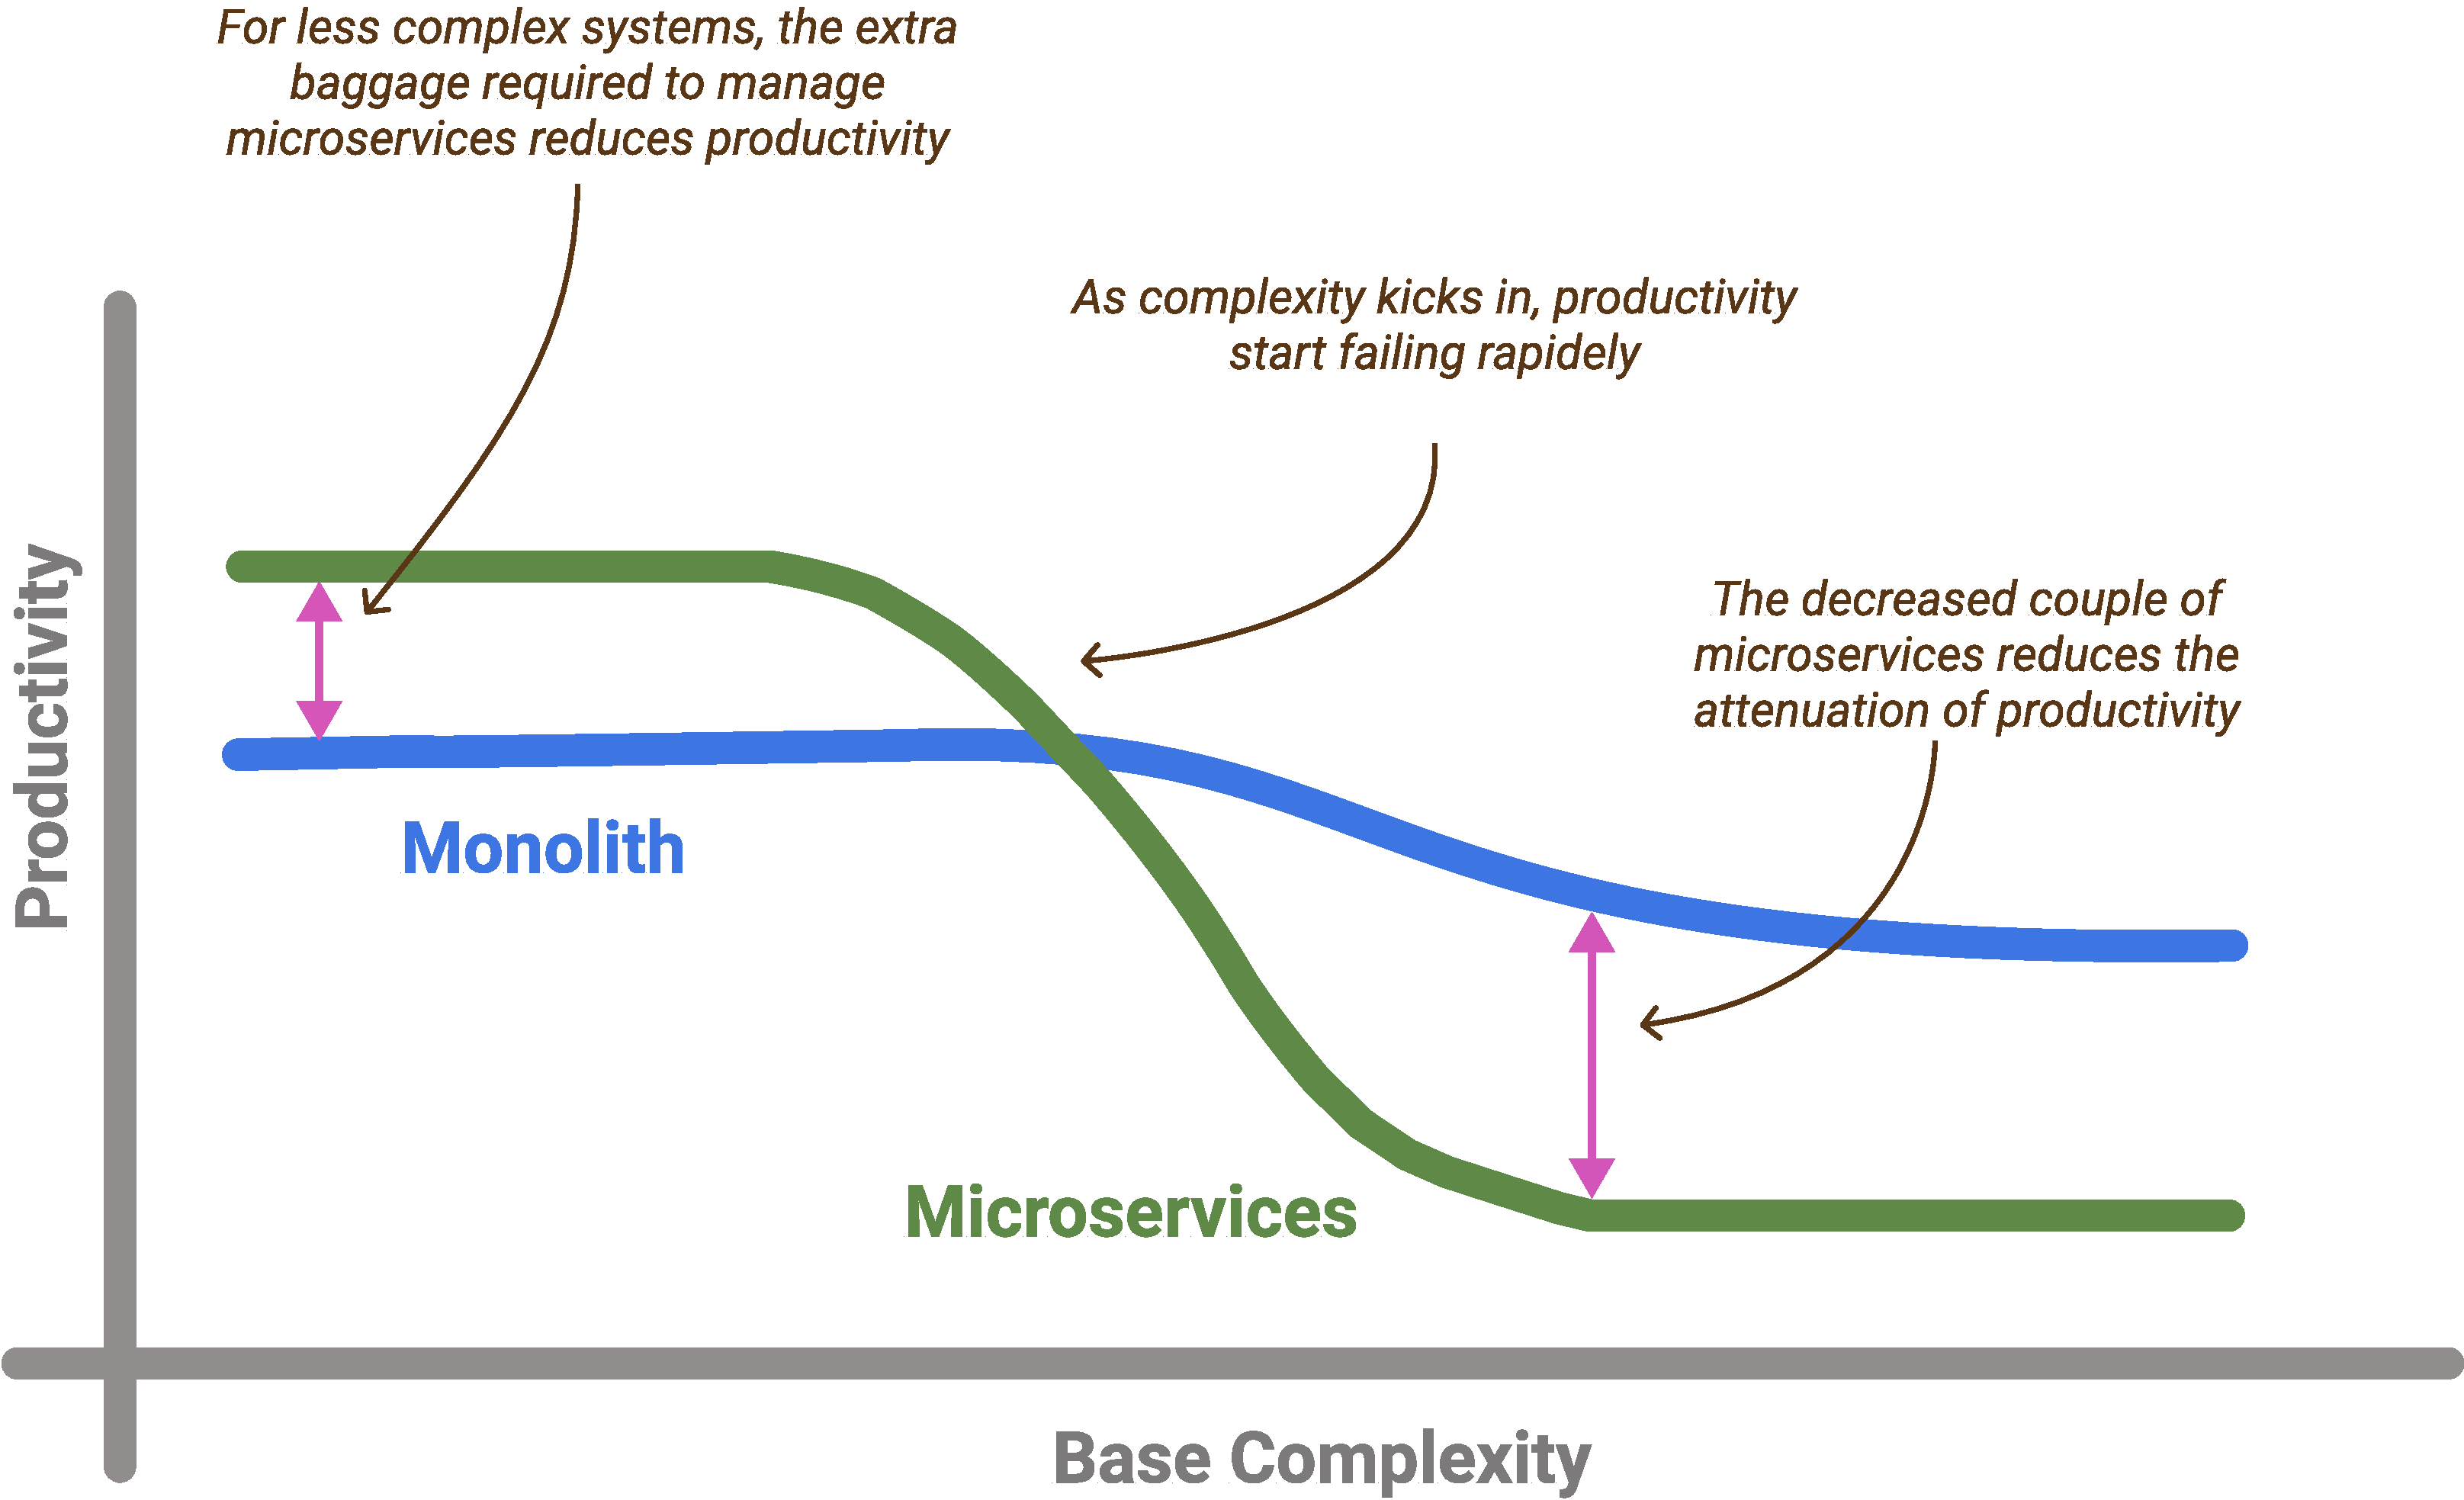
\includegraphics[width=1\textwidth]{Pictures/Monolith_vs_Microservice.pdf}
    \caption{Relation between system complexity and architectures. Source: https://martinfowler.com/bliki/MicroservicePremium.html}
    \label{fig:monolith_vs_microservice}
\end{figure}

In a logical multilayer architecture for an information system with an object-oriented design, the following four are the most common:

\begin{itemize} % source: https://en.wikipedia.org/wiki/Multitier_architecture#cite_note-5
    \item \textbf{Presentation Layer.} UI layer, view layer, presentation tier in multitier architecture.
    \item \textbf{Application Logic.} Service layer [\cite{ji2009intelligent, swetina2014toward}]
    or GRASP Controller Layer [\cite{okada2006vision}].
    \item \textbf{Business Logic.} Business logic layer, domain logic layer.
    \item \textbf{Data Access Layer.} Persistence layer, logging, networking, and other services which are required
    to support a particular business layer.
\end{itemize}

\begin{figure}[H]
    \centering
    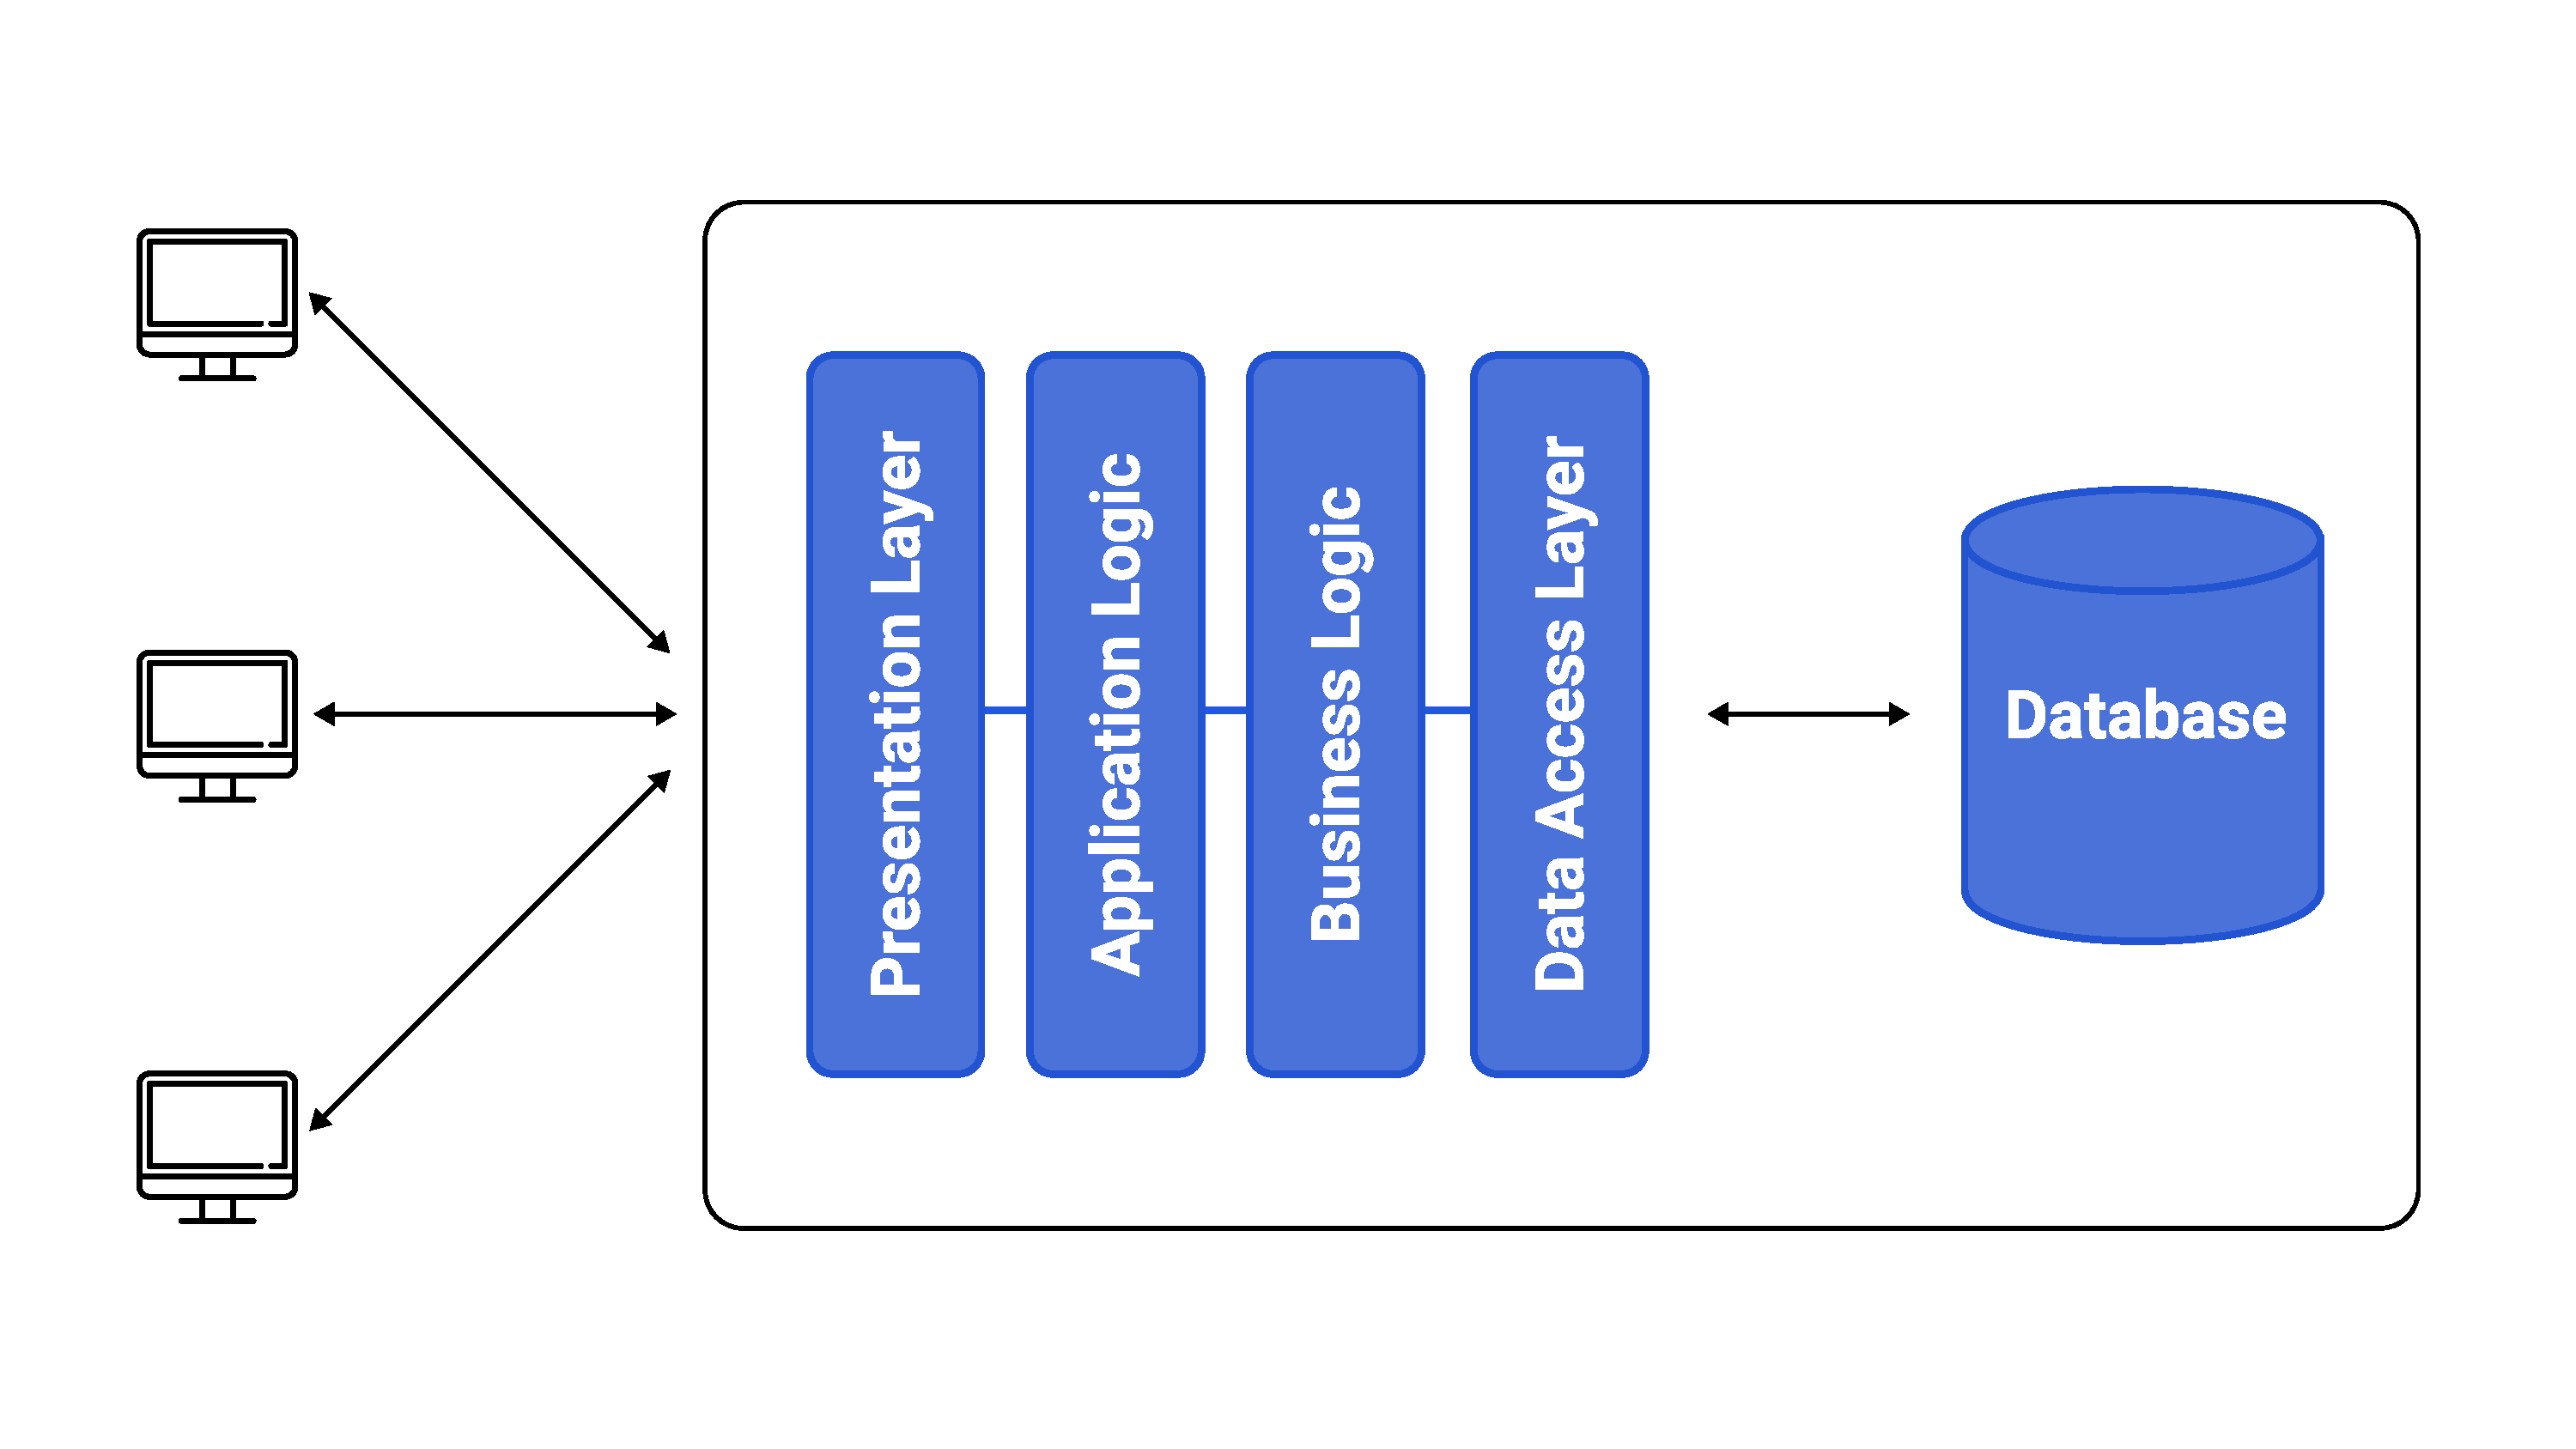
\includegraphics[width=1\textwidth]{Pictures/Monolith_architecture.pdf}
    \caption{Monolithic architecture diagram. Source: }\label{fig:figure2}
\end{figure}

The book Domain Driven Design describes some common uses for the above four layers, although its primary focus is the
domain layer [\cite{solvberg2010domain}].
If the application architecture has no explicit distinction between the business layer and the presentation layer,
then a traditional client-server model has been implemented.
The presentation layer is considered part of the business layer.
The more usual convention is that the application layer is considered a sublayer of the business layer,
typically encapsulating the API definition surfacing the supported business functionality.
The application/business layers can, in fact, be further subdivided to emphasize additional sub-layers of distinct
responsibility.
For example, if the model–view–presenter pattern is used, the presenter sublayer might be used as an additional layer
between the user interface layer and the business/application layer, as represented by the model sublayer.
Some also identify a separate layer called the business infrastructure layer, located between the business layer
and the infrastructure layer.
It's also sometimes called the \textit{low-level business layer} or the \textit{business services layer}.
The infrastructure layer can be partitioned into different levels, high-level or low-level technical services [\cite{dennis2018mcapl}].
Developers often focus on the persistence capabilities of the infrastructure layer and therefore only
talk about the persistence layer or the data access layer instead of an infrastructure layer or technical services layer.
In other words, the other kind of technical services are not always explicitly thought of as part of any particular layer.
A layer is on top of another, because it depends on it.
Every layer can exist without the layers above it, and requires the layers below it to function.
Another common view is that layers do not always strictly depend on only the adjacent layer below.
For example, in a relaxed layered system, a layer can also depend on all the layers below it [\cite{anon2014building}].
Relaxed layered system may be considered as opposed to a strict layered system.

\subsection{Monolith Architecture: Cons and Props}\label{subsec:monolith-architecture:-cons-and-props}

A monolith is built as a large system with a single code base and deployed as a single unit, usually behind a load balancer.
It typically consists of four major components: a user interface, business logic, a data interface and a database.
Monoliths offer several advantages, particularly when it comes to operational overhead requirements.
Here are some of those basic benefits:

\begin{itemize}
    \item \textbf{Simplicity.} Monolithic architectures are simple to build, test and deploy.
    These apps can scale horizontally, in one direction, by running several copies of the application behind a load balancer.
    Cross-cutting concerns: With a single codebase, monolithic apps can easily handle cross-cutting concerns, such as logging,
    configuration management and performance monitoring.
    Another advantage associated with the simplicity of monolithic apps is easier deployment.
    When it comes to monolithic applications, you do not have to handle many deployments – just one file or directory.
    \item \textbf{Performance.} Components in a monolith typically share memory which is faster than service-to-service
    communications using IPC [\cite{proctor1999linux}] or other mechanisms.
    \item \textbf{Easier debugging and testing.}
    In contrast to the microservices architecture, monolithic applications are much easier to debug and test.
    Since a monolithic app is a single indivisible unit, you can run end-to-end testing much faster.
    \item \textbf{Easier development.} As long as the monolithic approach is a standard way of building applications,
    any engineering team has the right knowledge and capabilities to develop a monolithic application.
\end{itemize}
But one major drawback of monolithic architectures is tight coupling.
Over time, monolithic components become tightly coupled and entangled.
This coupling effects management, scalability and continuous deployment.
Other cons that stem from tight coupling include:
\begin{itemize}
    \item \textbf{Understanding.} When a monolithic application scales up, it becomes too complicated to understand.
    Also, a complex system of code within one application is hard to manage.
    \item \textbf{Reliability.} An error in any of the modules in the application can bring the entire application down.
    \item \textbf{Updates.} Due to a single large codebase and tight coupling, the entire application would have to deploy
    for each update.
    \item \textbf{Technology stack.} A monolithic application must use the same technology stack throughout.
    Changes to the technology stack are expensive, both in terms of the time and cost involved.
    \item \textbf{Scalability.} You cannot scale components independently, only the whole application.
\end{itemize}

\subsection{Decoupling Monolith using CQRS}\label{subsec:decoupling-monolith-using-cqrs}
As it stated in previous section, monolithic architecture provides a quite strong coupling between application
components.
Moreover, as monolith grow horizontally, its services layer grows as well.
This process leads to very huge code base which is very difficult to support and extend.
We attach the following
\href{https://github.com/smartstore/SmartStoreNET/blob/4.x/src/Presentation/SmartStore.Web/Controllers/CatalogHelper.cs}
{link}
as an example of such approach.
To avoid the natural results of monolithic architecture, that are huge classes for thousands lines, we have to dive into
design patterns [\cite{rising1998design}].
Precisely, the mediator design pattern would help to decouple the service layer from presentation layer.
Mediator -- is a behavioral design pattern [\cite{rasche2016building}] that lets you reduce chaotic dependencies between objects.
The pattern restricts direct communications between the objects and forces them to collaborate only via a mediator object.
In other words, mediator allows the communication between two entities, such that entities doesn't know each other.
The Mediator pattern suggests that you should cease all direct communication between the components which you want to make
independent of each other.
Instead, these components must collaborate indirectly, by calling a special mediator object that redirects the calls to
appropriate components.
As a result, the components depend only on a single mediator class instead of being coupled to dozens of their colleagues.
In context of .NET platform there are multiple implementation of the Mediator, the most widely known and used is the
\href{https://github.com/jbogard/MediatR}{MediatR}, which we use in our project.
Another, yet popular approach is the CQRS, which stands for Command-Query Responsibility Segregation.
In brief, it stands that read (query) and write (command) requests should be segregated by their responsibilities.
The CQRS approach in couple with Mediator greatly helps to solve the coupling problem of the monolith architecture.
So what is CQRS precisely?
According to \href{https://martinfowler.com/bliki/CQRS.html}{Martin Fowler},
it is a pattern that first described by Greg Young [\cite{young2010cqrs}].
At its heart is the notion that you can use a different model to update information than the model you use to read information.
For some situations, this separation can be valuable, but beware that for most systems CQRS adds risky complexity.
The mainstream approach people use for interacting with an information system is to treat it as a CRUD datastore.
By this meant that we have mental model of some record structure where we can create new records, read records,
update existing records, and delete records when we're done with them.
In the simplest case, our interactions are all about storing and retrieving these records.
As our needs become more sophisticated we steadily move away from that model.
We may want to look at the information in a different way to the record store, perhaps collapsing multiple records into one,
or forming virtual records by combining information for different places.
On the update side we may find validation rules that only allow certain combinations of data to be stored, or may even infer
data to be stored that's different from that we provide.
For instance, the idea of command-query segregation is displayed at the following image

\begin{figure}[H]
    \centering
    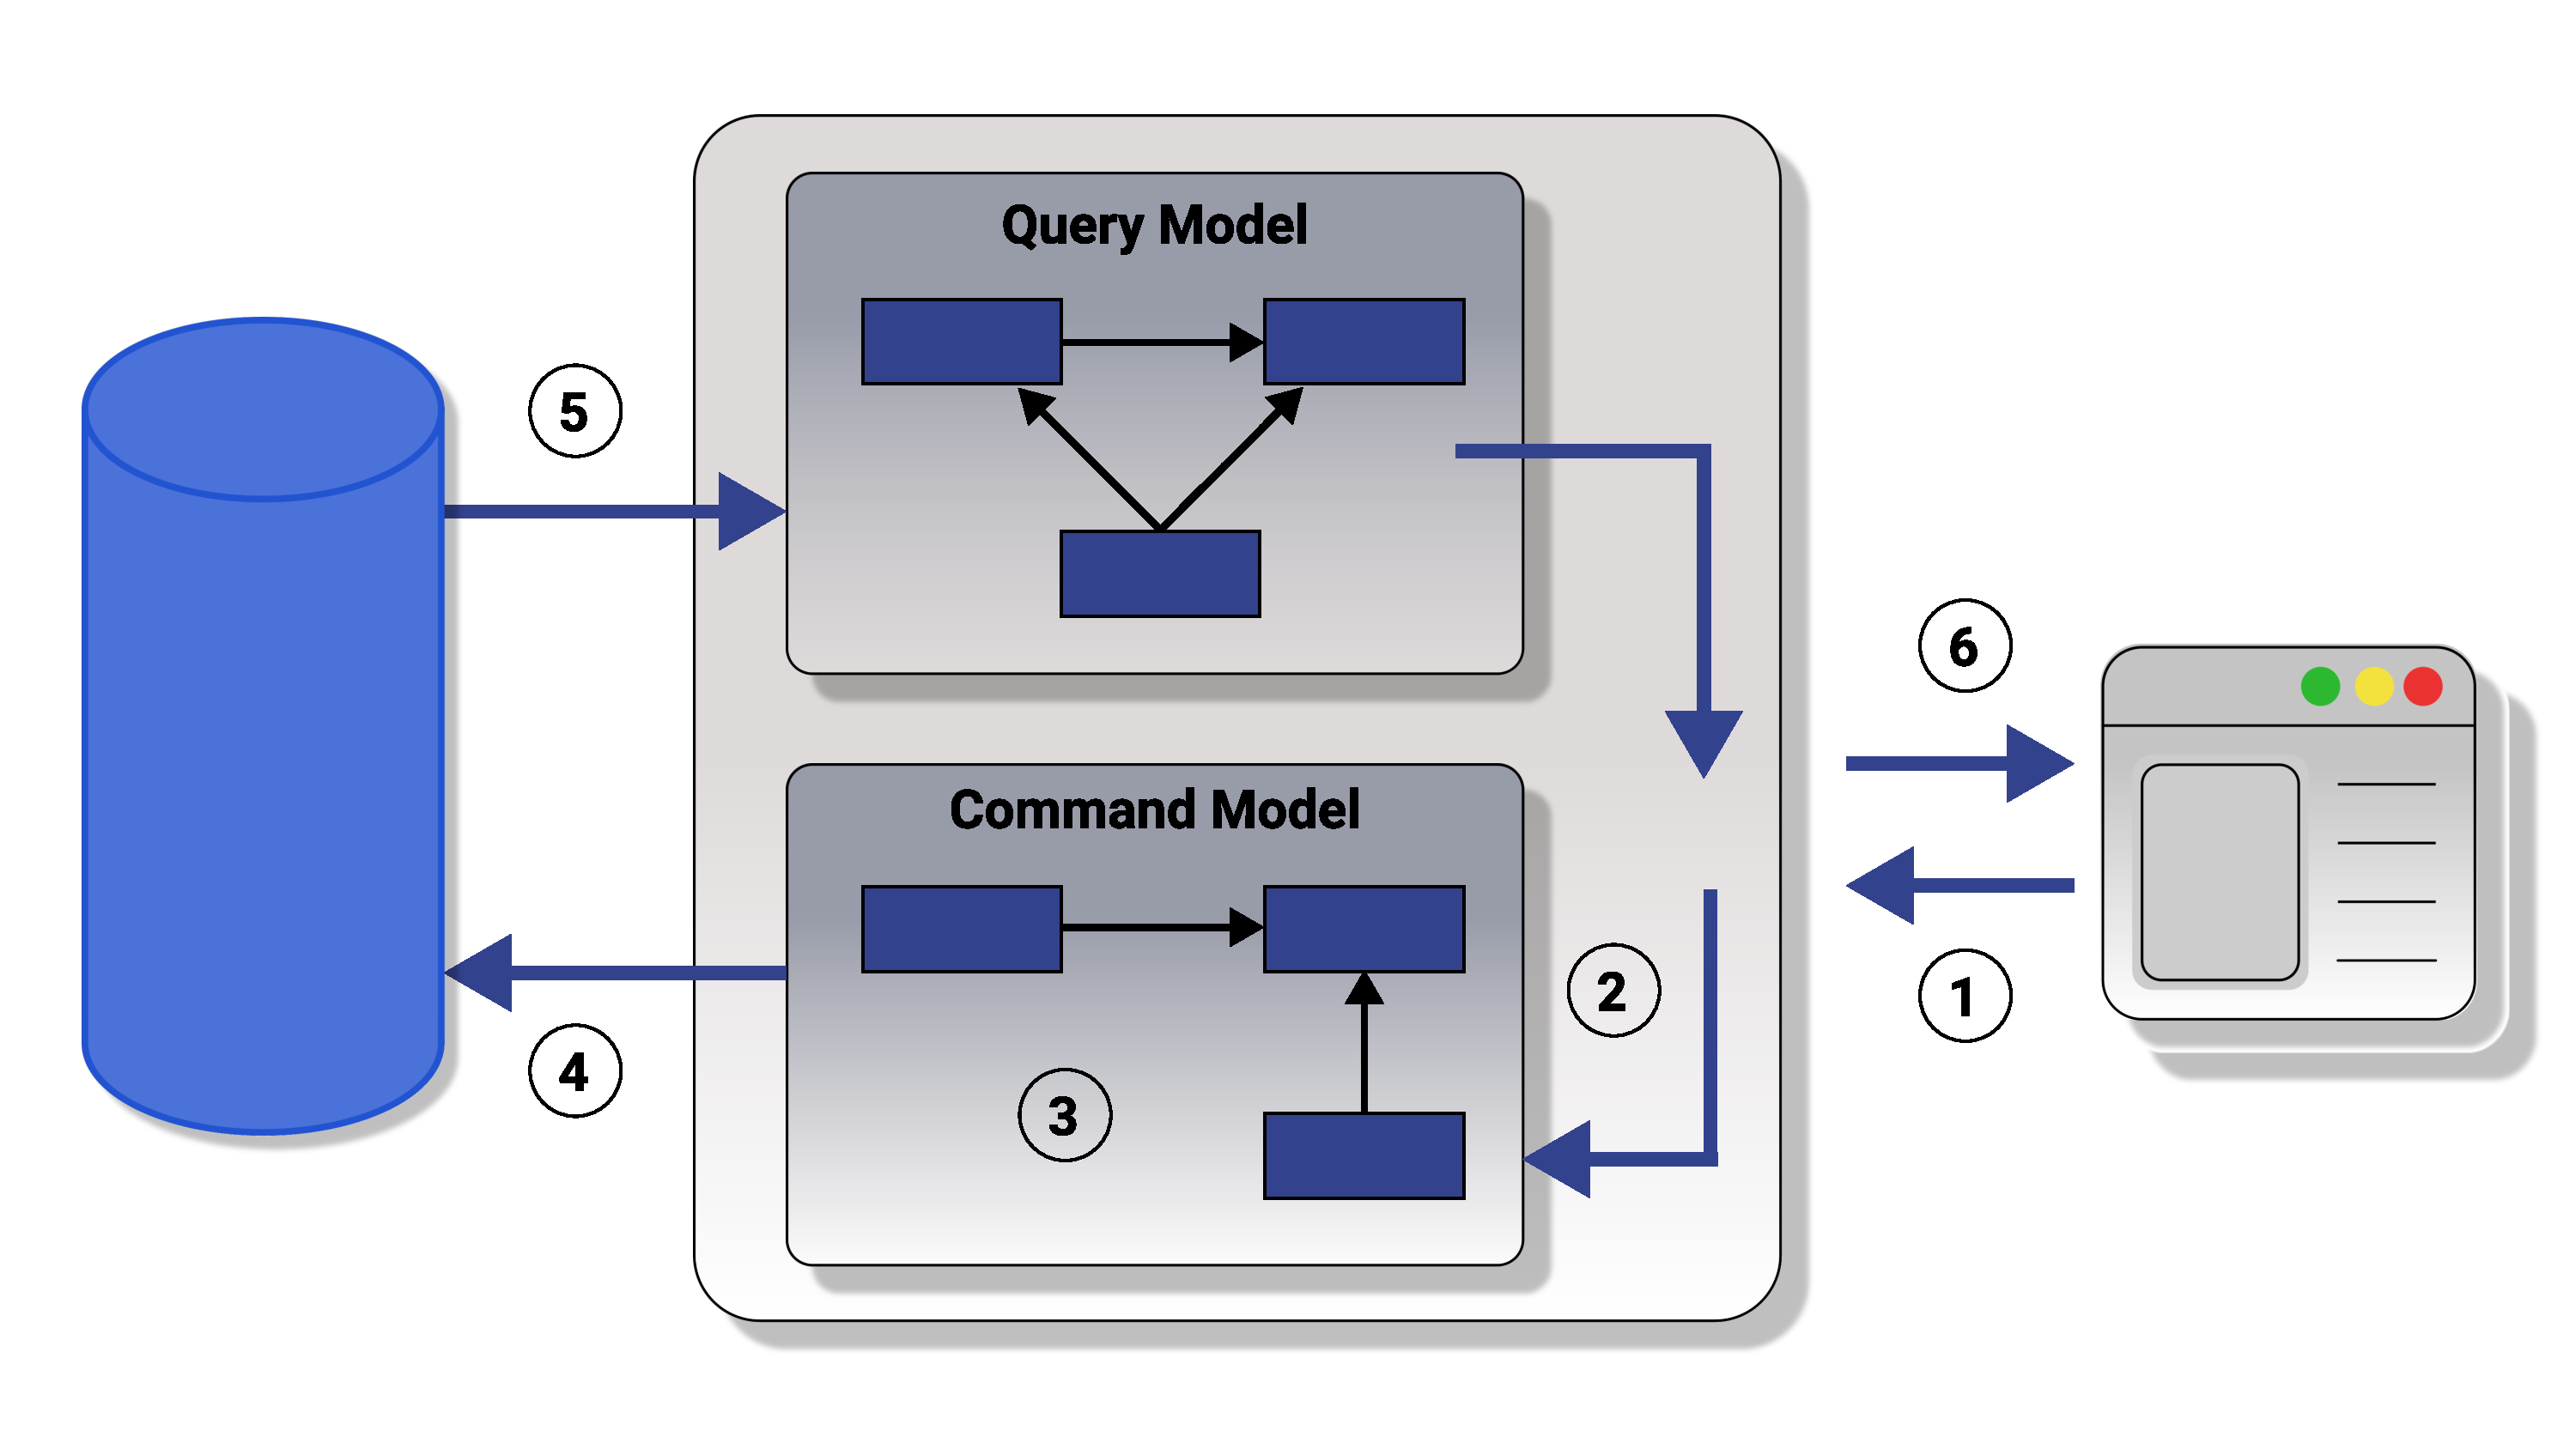
\includegraphics[width=1\textwidth]{Pictures/cqrs.pdf}
    \caption{CQRS Conceptual diagram. Source: https://martinfowler.com/bliki/CQRS.html}\label{fig:figure}
\end{figure}

\begin{enumerate}
    \item User makes a change in UI\@.
    \item Application routes information to command model.
    \item Command model executes validation and business logic.
    \item Command model updates the database.
    \item Query model reads from database.
    \item Query service update presentation from query model.
\end{enumerate}

Despite these benefits, you should be very cautious about using CQRS\@.
Many information systems fit well with the notion of an information base that is updated in the same way that it's read,
adding CQRS to such a system can add significant complexity.
I've certainly seen cases where it's made a significant drag on productivity, adding an unwarranted amount of risk to the
project, even in the hands of a capable team.
So while CQRS is a pattern that's good to have in the toolbox, beware that it is difficult to use well and you can easily
chop off important bits if you mishandle it.

As a short conclusion, we may state that CQRS and Mediator pattern will not entirely solve the coupling problems the monolith,
however will make project much more simplistic and intuitively understood.
It is worth to keep is simple,
even relatively simple project may grow to the sizes of universe without proper architectural solutions.

\subsection{Database Structure and related comments}\label{subsec:database-structure-and-related-comments}
As a next topic to uncover goes the one related to the database structure.
Proper database structure is to be of very high priority, since it influences on the project as a whole,
starting from performance point of view and many other aspects.
When we say performance, we mean such a design of database that there is an opportunity to include required indexes,
depending on regularity of any particular request.
So, as the main topic of current thesis is implementation of Instant messaging system, we can list the following
general entities to be added to database schema.

\begin{itemize}
    \item \textbf{Users.} Table stores information about user.
    Table contains following columns:
    \begin{itemize}
        \item Id VARCHAR(36) -- Id of the user, primary key, GUID\@.
        \item UserName VARCHAR(50) -- Unique Username.
        \item NormalizedUserName VARCHAR(50) -- Unique Username in upper case.
        \item DisplayName VARCHAR(50) -- Name of the user, displayed to others.
        \item Bio VARCHAR(250) -- User's short biography, visible to others.
        \item Image VARCHAR(36) -- User's profile picture, visible to others.
        \item Email VARCHAR(120) -- User's email address, not public.
        \item EmailConfirmed BOOLEAN -- Flag that indicates if user has confirmed his email address.
        \item PhoneNumber VARCHAR(50) -- User's phone number.
        \item PhoneNumberConfirmed BOOLEAN -- Flag that indicates if user has confirmed his phone number.
        \item PhoneVerificationCode INTEGER -- Code sent to user in order to confirm phone number.
        \item PasswordHash VARCHAR(60) -- Hashed password.
        \item CreatedAt DATETIME -- Indicates the date and time user has been registered.
        \item UpdatedAt DATETIME -- Indicates the date and time user has updated his record.
    \end{itemize}
    \item \textbf{User Personal Information.} Table stores additional but not required info about user.
    Relation one-to-one with Users, foreign key is UserId, GUID\@.
    Table contains following columns:
    \begin{itemize}
        \item UserId VARCHAR(36) -- Foreign key to the Users table, GUID\@.
        \item FirstName VARCHAR(120) -- First name of user.
        \item LastName VARCHAR(120) -- Last name of user.
        \item BirthDay DATETIME -- Birth day of user.
        \item WebSite VARCHAR(120) -- Web site of user.
        \item Address VARCHAR(120) -- Residence address of user.
        \item Facebook VARCHAR(120) -- Facebook nickname of user.
        \item Twitter VARCHAR(120) -- Twitter nickname of user.
        \item Instagram VARCHAR(120) -- Instagram nickname of user.
        \item LinkedIn VARCHAR(120) -- LinkedIn nickname of user.
        \item ProfilePicture VARCHAR(36) -- Avatar of user.
    \end{itemize}
    \item \textbf{UserContacts.} Table stores the contacts of current user.
    Relation between tables Users and UserContacts is one-to-many, foreign key UserId.
    Table contains following columns:
    \begin{itemize}
        \item ContactId VARCHAR(36) -- Id of current user's contact, GUID\@.
        \item UserId VARCHAR(36) -- Id of current user, GUID\@.
    \end{itemize}
    \item \textbf{Chats.} In order to communicate with other people it is essentially to have a chat room.
    Our implementation provides chat rooms of the four types.
    Direct chat -- chat room between only two members.
    Public channel -- chat room for multiple members, each member can send and read messages.\ It displayed in search results.
    Readonly channel -- channel for multiple members, however only the owner can send messages.\ It displayed in search results.
    Private channel -- channel for multiple members, can be joined only by invite link.
    Each user can have a numerous various chats, however, each chat has a multiple members, at least 2 as the case of direct chat.
    Therefore, we consider a many-to-many relation between user and chats via intermediate table UserChats.
    We discuss UserChats relation in foregoing part.
    Continuing with Chats table, it contains the following columns:
    \begin{itemize}
        \item Id VARCHAR(36) -- Id of the chat, primary key, GUID.
        \item ChatInfoId VARCHAR(36) -- Since we have a four types of channels, which has a common subset of data,
        the different data is moved to another table, so it could be joined depending on chat type.
        For instance, any chat type except direct one would require to join additional data in order to display the chat properly.
        \item Title VARCHAR(50) -- Simply, the title of the chat.
        \item Image VARCHAR(36) -- Picture of the chat.\ Displayed in search results etc.
        \item ChatType ENUM -- The type of the chat, e.g direct chat, public channel, readonly channel, private channel.
        \item CreatedAt DATETIME -- Indicates the date and time chat has been created.
        \item UpdatedAt DATETIME -- Indicates the date and time chat has been updated.
    \end{itemize}
    \item \textbf{UserChats.} Table that considered as composite key of the many-to-many relation between Users and Chats tables.
    Over that, contains an enum value that indicates user's role in the chat.
    We assume the following user roles in the system:
    \begin{itemize}
        \item Owner -- the creator of the chat.
        Has an ultimate privileges.
        \item Administrator -- designated by the owner user, which has adjustable privileges.
        \item Moderator -- designated by administrator user, which has adjustable privileges.
        \item User -- default role assigned to the user on join the chat.
    \end{itemize}
    Despite that, the UserChats table contains the following columns:
    \begin{itemize}
        \item ChatId VARCHAR(36) -- Foreign key to the Chats table, GUID\@.
        \item UserId VARCHAR(36) -- Foreign key to the Users table, GUID\@.
        \item RoleId ENUM -- Indicates the user role in the chat, e.g Owner, Administrator, Moderator, User.
    \end{itemize}
    \item \textbf{Chat Info.} Table contains additional data related to the chat.
    This table is created since that we have four types of chats, namely, direct chat, public channel,
    readonly channel, private channel.
    These four types has a common data between each other.
    Common data between chat types is Chats table itself.
    One would advise to store the chats in a single table per chat type, however it is very costly approach, since there
    would be at least four joins per request.
    Note that every chat type except direct chat requires an additional data to be displayed, that is Chat Info.
    Contains following columns:
    \begin{itemize}
        \item Id VARCHAR(36) -- Id of the chat information, primary key, GUID\@.
        \item Description VARCHAR(120) -- Description of the chat.
        \item Tag VARCHAR(20) -- Unique identifier of the chat.
        \item MembersCount INTEGER -- Count of members in the chat.
    \end{itemize}
    \item \textbf{Messages.} Table that keeps messages and related data.
    Each chat has a multiple messages, however one message must belong only to single and defined chat,
    therefore relation between Chats and Messages is one-to-many, foreign key ChatId.
    From other side, each User has a multiple messages, however single message should belong to single author,
    therefore, we consider one-to-mane relation between Users and Messages, foreign key UserId.
    Messages table contains following columns:
    \begin{itemize}
        \item Id VARCHAR(36) -- Id of the message, primary key, GUID\@.
        \item ChatId VARCHAR(36) -- Foreign key to the Chats table, GUID\@.
        \item UserId VARCHAR(36) -- Foreign key to the Users table, GUID\@.
        \item Content VARCHAR(300) -- Content of the message.
        \item IsRead BOOLEAN -- Indicates whenever message has been read by another user.
        \item CreateAt DATETIME -- Time when the message has been created.
        \item UpdatedAt DATETIME -- Time when the message has been updated.
    \end{itemize}
    \item \textbf{Refresh Tokens.} Table stores refresh tokens.
    \begin{itemize}
        \item Id VARCHAR(36) -- Id of the token, primary key, GUID\@.
        \item UserId VARCHAR(39) -- Foreign key to the Users table, GUID\@.
        \item RefreshToken VARCHAR(60) -- Refresh token itself.
        \item Expires DATETIME -- Expiration date of refresh token.
        \item CreatedAt DATETIME -- Date when token has been created.
    \end{itemize}
\end{itemize}
Following diagram demonstrates the database structure.
\begin{figure}[H]
    \centering
    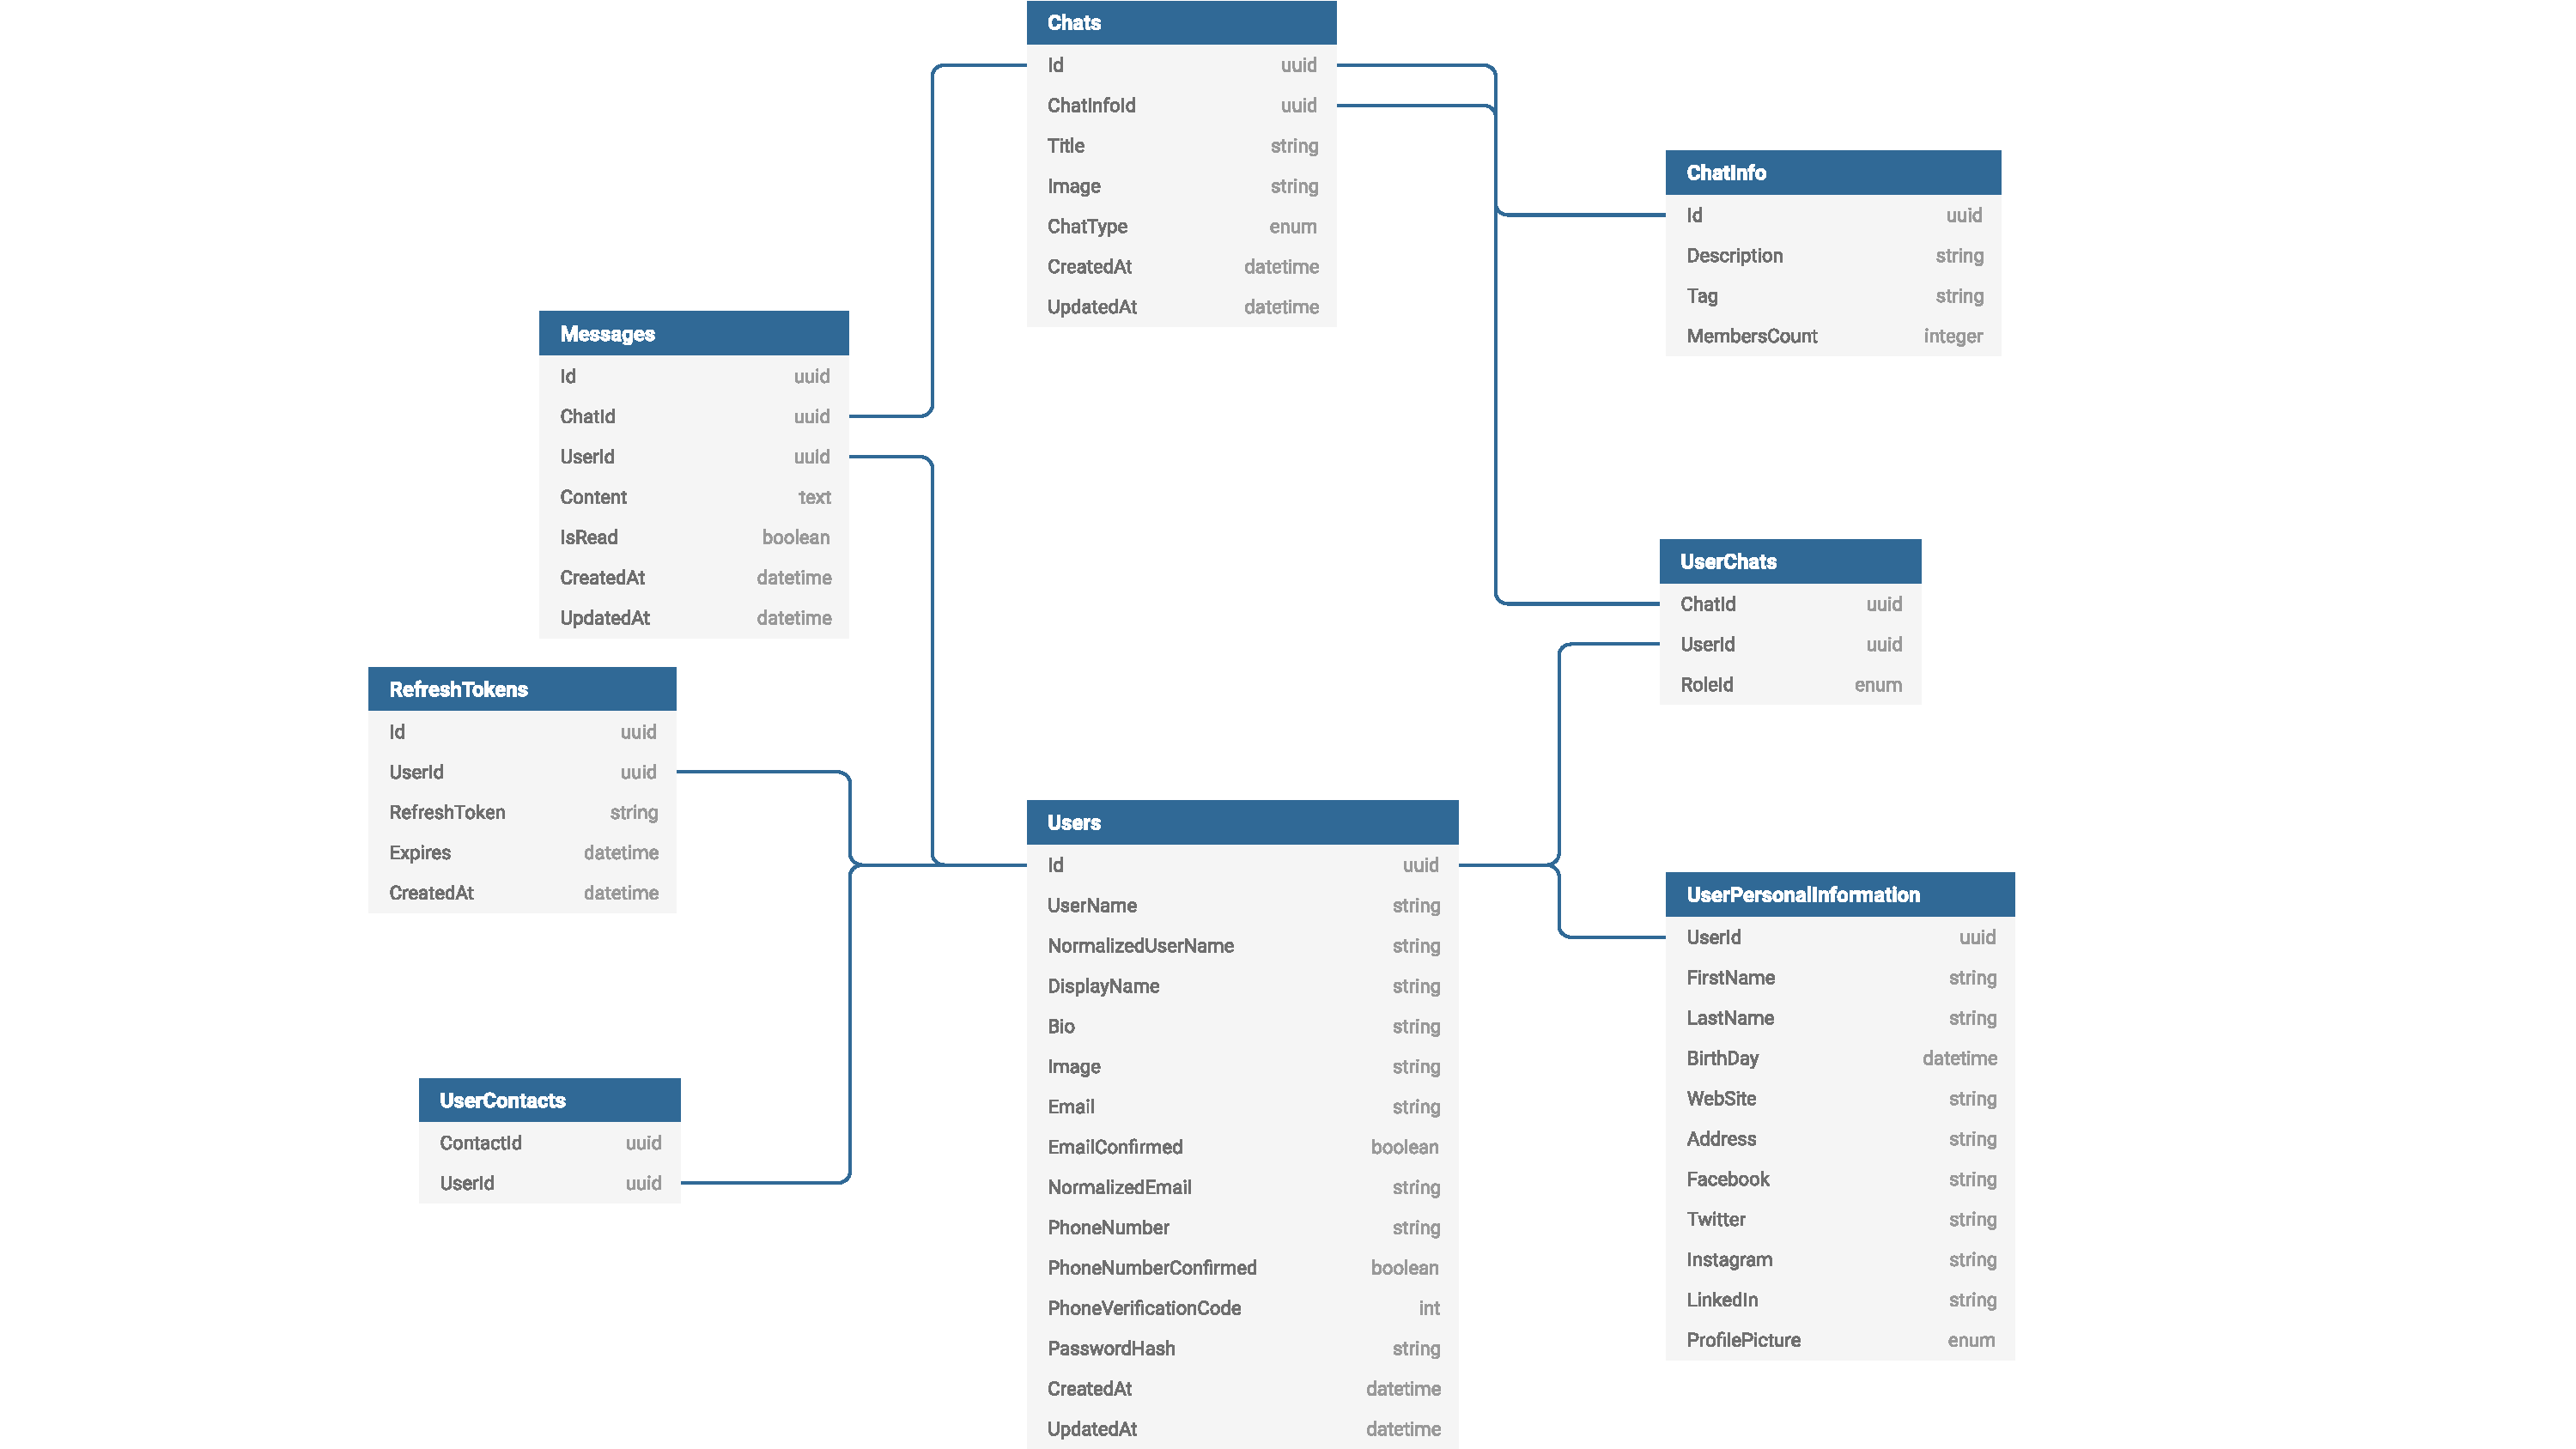
\includegraphics[width=1.2\textwidth]{Pictures/DB_diagram}
    \caption{Database diagram}\label{fig:figure5}
\end{figure}
Over whole data entities, we prefer to use universally unique identifier (UUID) or namely globally unique identifier (GUID),
a 128-bit label used for information in computer systems [\cite{leach2005universally}].
Simply, because it does not force us to keep a sequence on database side.
Sequence -- is a special entity provided in PostgreSQL relational databases.
It is responsible for generating unique values and sometimes causes a problems during migration of the database.
But still, are GUID identifiers are really always unique?
Well, each generated GUID is not guaranteed to be unique, the total number of unique keys $2^{128}$ or $3.4 \times 10^{38}$
is so large that the probability of the same number being generated twice is very small.
For example, consider the observable universe, which contains about $5 \times 10^{22}$ stars.
Every star could then have $6.8 \times 10^{15}$ universally unique GUIDs.
If you are scared of the same GUID values then put two of them next to each other.
If you are too paranoid then put three [\cite{GUIDSo}].

% source: https://en.wikipedia.org/wiki/HTTPS


\section{Discussion on HTTPS Protocol}\label{sec:discussion-on-https-protocol}
HTTPS stands for Hypertext Transfer Protocol Secure.
HTTPS is an extension of the Hypertext Transfer Protocol.
It is used for secure communication over a computer network,
and is widely used on the Internet [\cite{lam2000secure, karayiannis2019implementing}].
In HTTPS, the communication protocol is encrypted using Transport Layer Security [\cite{turner2014transport}]
or, formerly, Secure Sockets Layer [\cite{weaver2006secure}].
The protocol is therefore also referred to as HTTP over TLS or HTTP over SSL\@.
The principal motivations for HTTPS are authentication of the accessed website, and protection of the privacy and integrity
of the exchanged data while in transit.
It protects against \textit{man-in-the-middle attacks}.
The bidirectional encryption of communications between a client and server protects the communications against
eavesdropping and tampering [\cite{mayer2016tlscompare, jiang2019physical}].
The authentication aspect of HTTPS requires a trusted third party to sign server-side digital certificates.
This was historically an expensive operation, which meant fully authenticated HTTPS connections were usually found only
on secured payment transaction services and other secured corporate information systems on the World Wide Web.
In 2016, a campaign by the Electronic Frontier Foundation with the support of web browser developers led to the protocol
becoming more prevalent [\cite{he2014shadowcrypt}].
HTTPS is now used more often by web users than the original non-secure HTTP, primarily to protect
page authenticity on all types of websites;
secure accounts;
and to keep user communications, identity, and web browsing private [\cite{rescorla2000rfc2818}].

\subsection{What is an SSL Certificate?}\label{subsec:what-is-an-ssl-certificate?}
SSL certificates are what enable websites to move from HTTP to HTTPS, which is more secure.
An SSL certificate is a data file hosted in a website's origin server.
SSL certificates make SSL/TLS encryption possible, and they contain the website's public key and the website's identity,
along with related information.
Devices attempting to communicate with the origin server will reference this file to obtain the public key and verify
the server's identity.
The private key is kept secret and secure.
SSL certificates include:
\begin{itemize}
    \item The domain name that the certificate was issued for
    \item Which person, organization, or device it was issued to
    \item Which certificate authority issued it
    \item The certificate authority's digital signature
    \item Associated sub-domains
    \item Issue date of the certificate
    \item Expiration date of the certificate
    \item The public key (the private key is kept secret)
\end{itemize}
The public and private keys used for SSL are essentially long strings of characters used for encrypting and decrypting data.
Data encrypted with the public key can only be decrypted with the private key, and vice versa.
\begin{figure}[H]
    \centering
    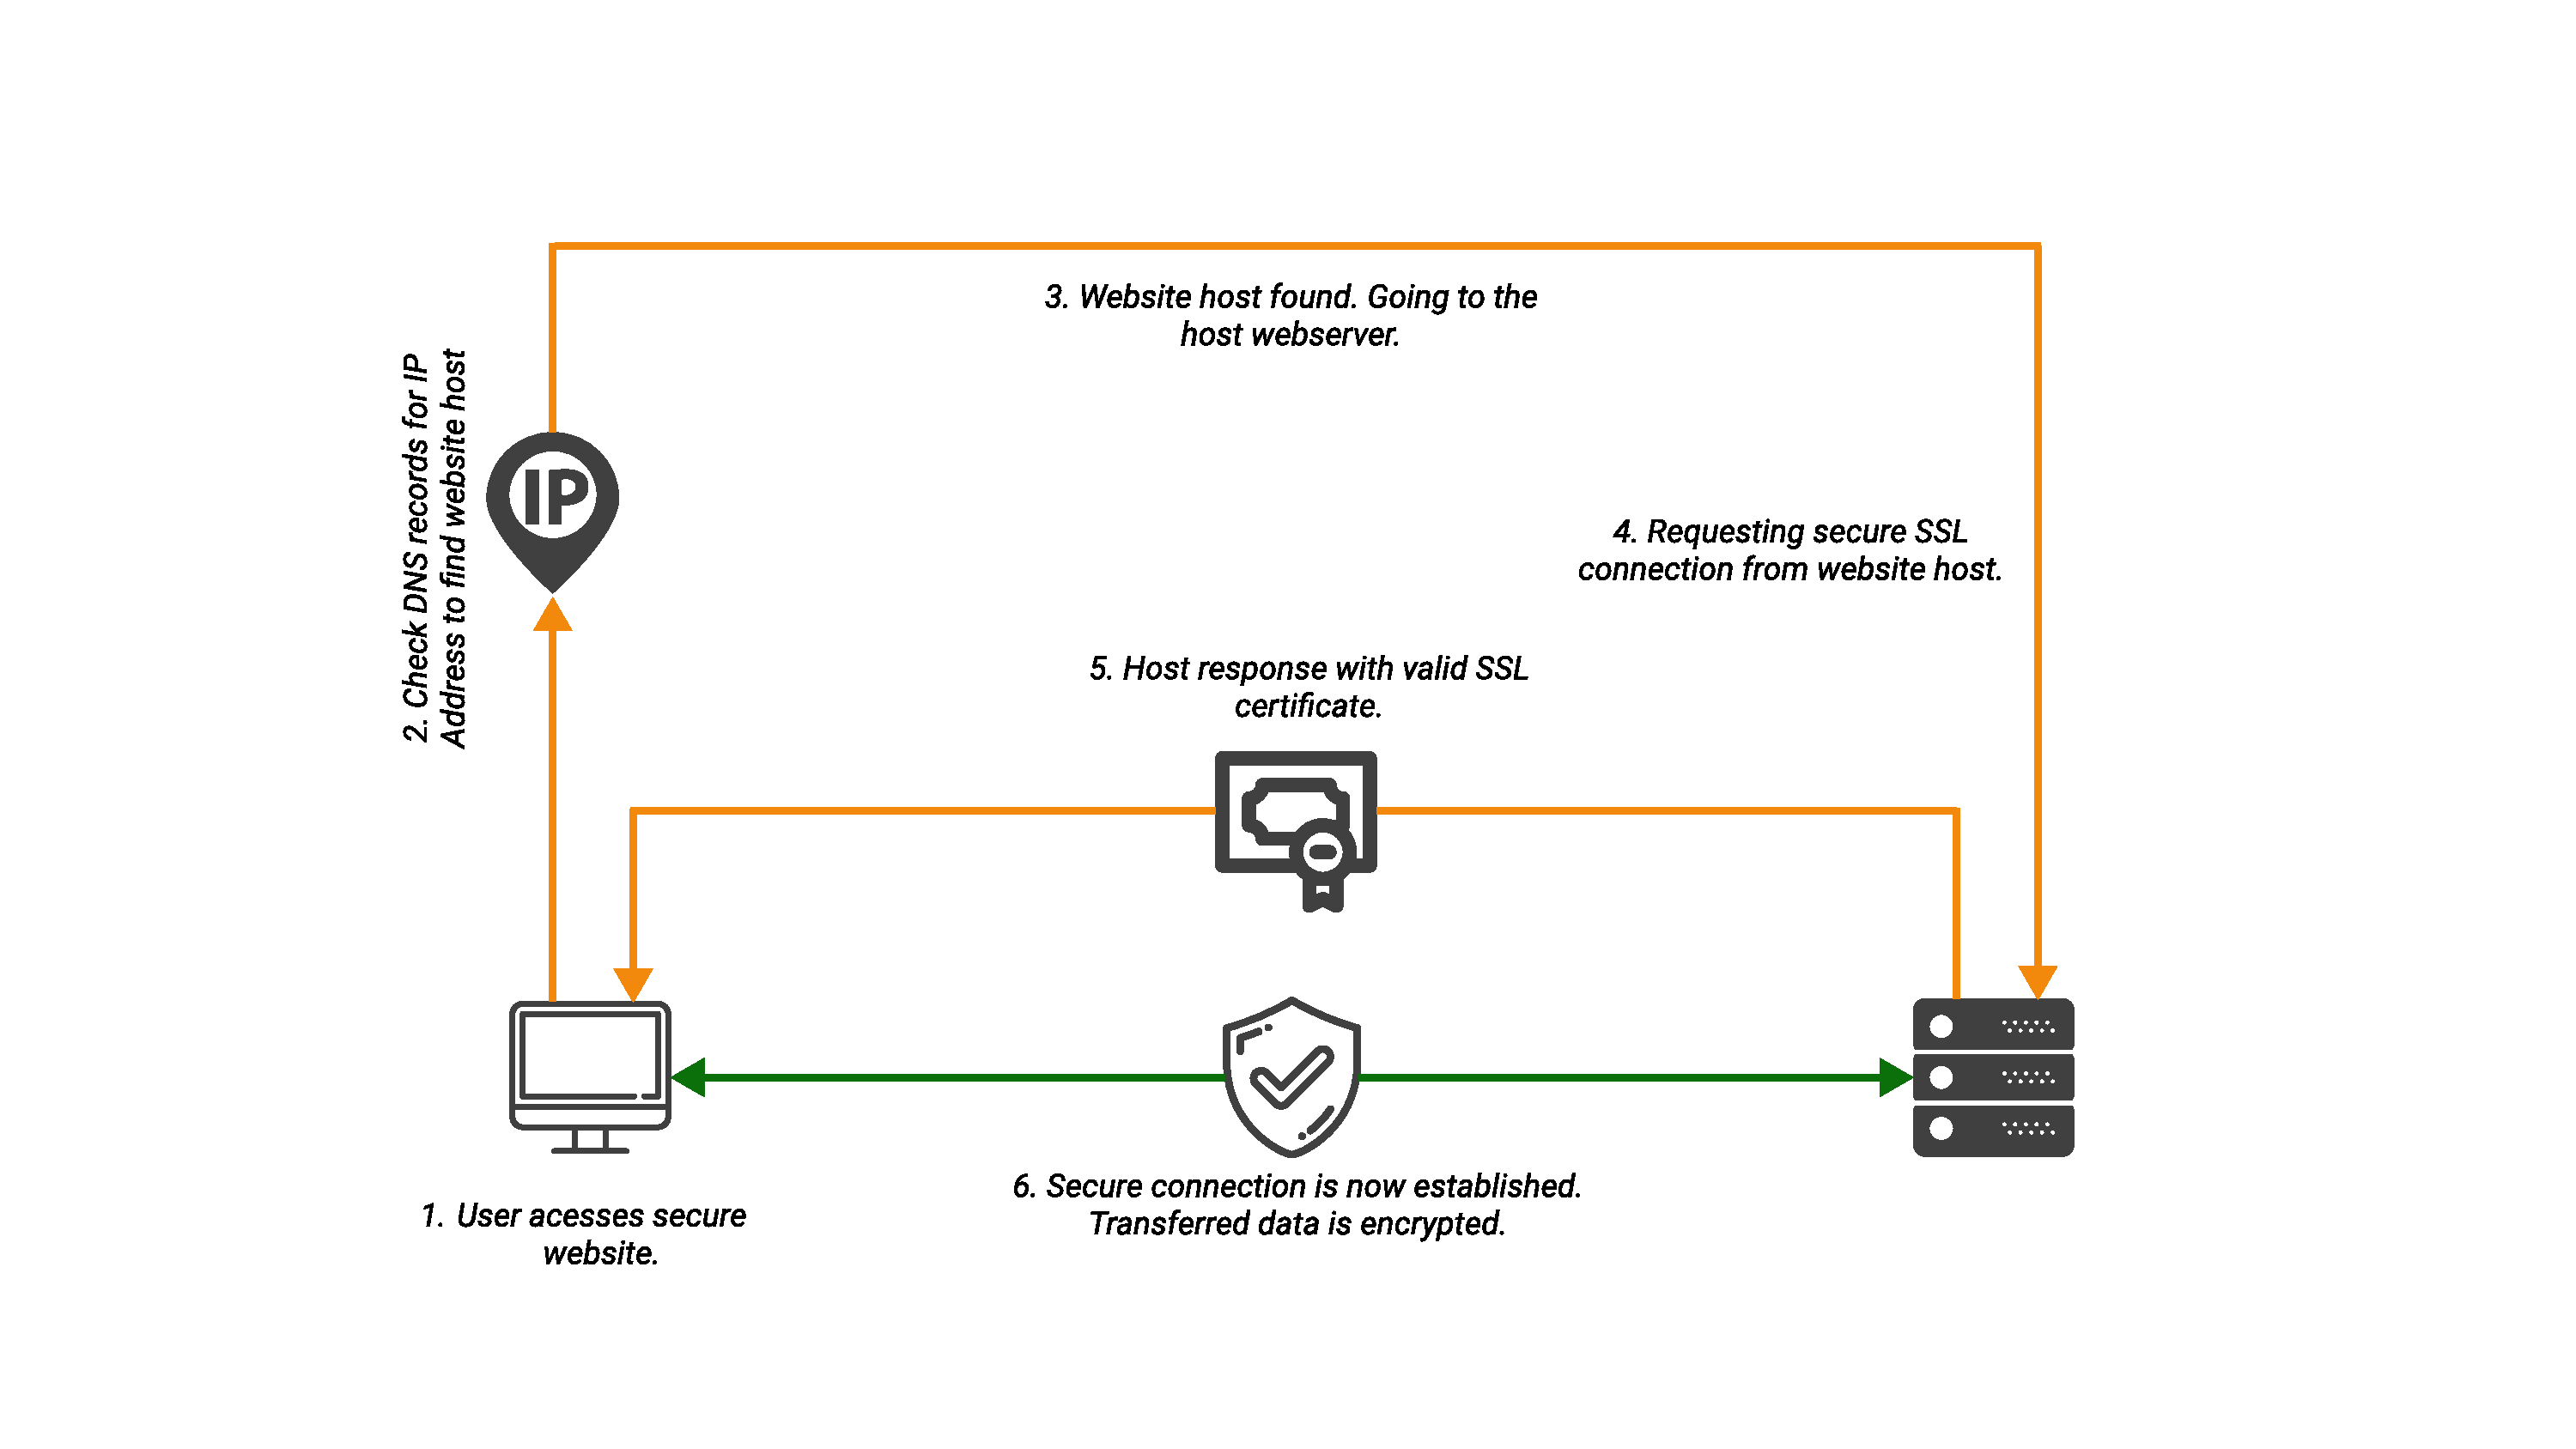
\includegraphics[width=1\textwidth]{Pictures/HTTPS_Flow}
    \caption{HTTPS flow diagram. Source: }\label{fig:figure6}
\end{figure}

\subsection{Discussion on E2E Encryption over HTTPS Protocol}\label{subsec:discussion-on-e2e-encryption-over-https-protocol}
Discuss here about why it is useless to implement E2E encryption in web version,
however is ok to implement for mobile one [\cite{JsMathRandom, E2eVsTLS}].
Answer the questions:
\begin{itemize}
    \item What is End-to-End (E2E) Encryption?
    \item How it is used in telegram?
    \item Does it make sense to implement it for web version?
    \item Does it make sense to implement it for mobile version?
    \item Why is it not worth that to implement E2E for web version?
\end{itemize}
\section{Diffie-Hellman Key Exchange}\label{sec:diffie-hellman-key-exchange}
Diffie–Hellman key exchange [\cite{li2010research}] is a method of securely exchanging cryptographic keys over a public channel
and was one of the first public-key protocols
as conceived by Ralph Merkle and named after Whitefield Diffie and Martin Hellman.
DH is one of the earliest practical examples of public key exchange implemented within the field of cryptography.
Published in 1976 by Diffie and Hellman, this is the earliest publicly known work that proposed the idea of a private
key and a corresponding public key.
Traditionally, secure encrypted communication between two parties required that they first exchange keys by some secure physical means,
such as paper key lists transported by a trusted courier.
The Diffie–Hellman key exchange method allows two parties that have no prior knowledge of
each other to jointly establish a shared secret key over an insecure channel.
This key can then be used to encrypt subsequent communications using a symmetric-key cipher.
Although Diffie–Hellman key agreement itself is a non-authenticated key-agreement protocol, it provides the basis for a
variety of authenticated protocols, and is used to provide forward secrecy in Transport Layer Security's ephemeral modes,
referred to as EDH or DHE [\cite{ahirwal2013elliptic}] depending on the cipher suite.

Diffie–Hellman key exchange establishes a shared secret between two parties that can be used for secret communication
for exchanging data over a public network.
An analogy illustrates the concept of public key exchange by using colors instead of very large numbers:
\begin{figure}[H]
    \centering
    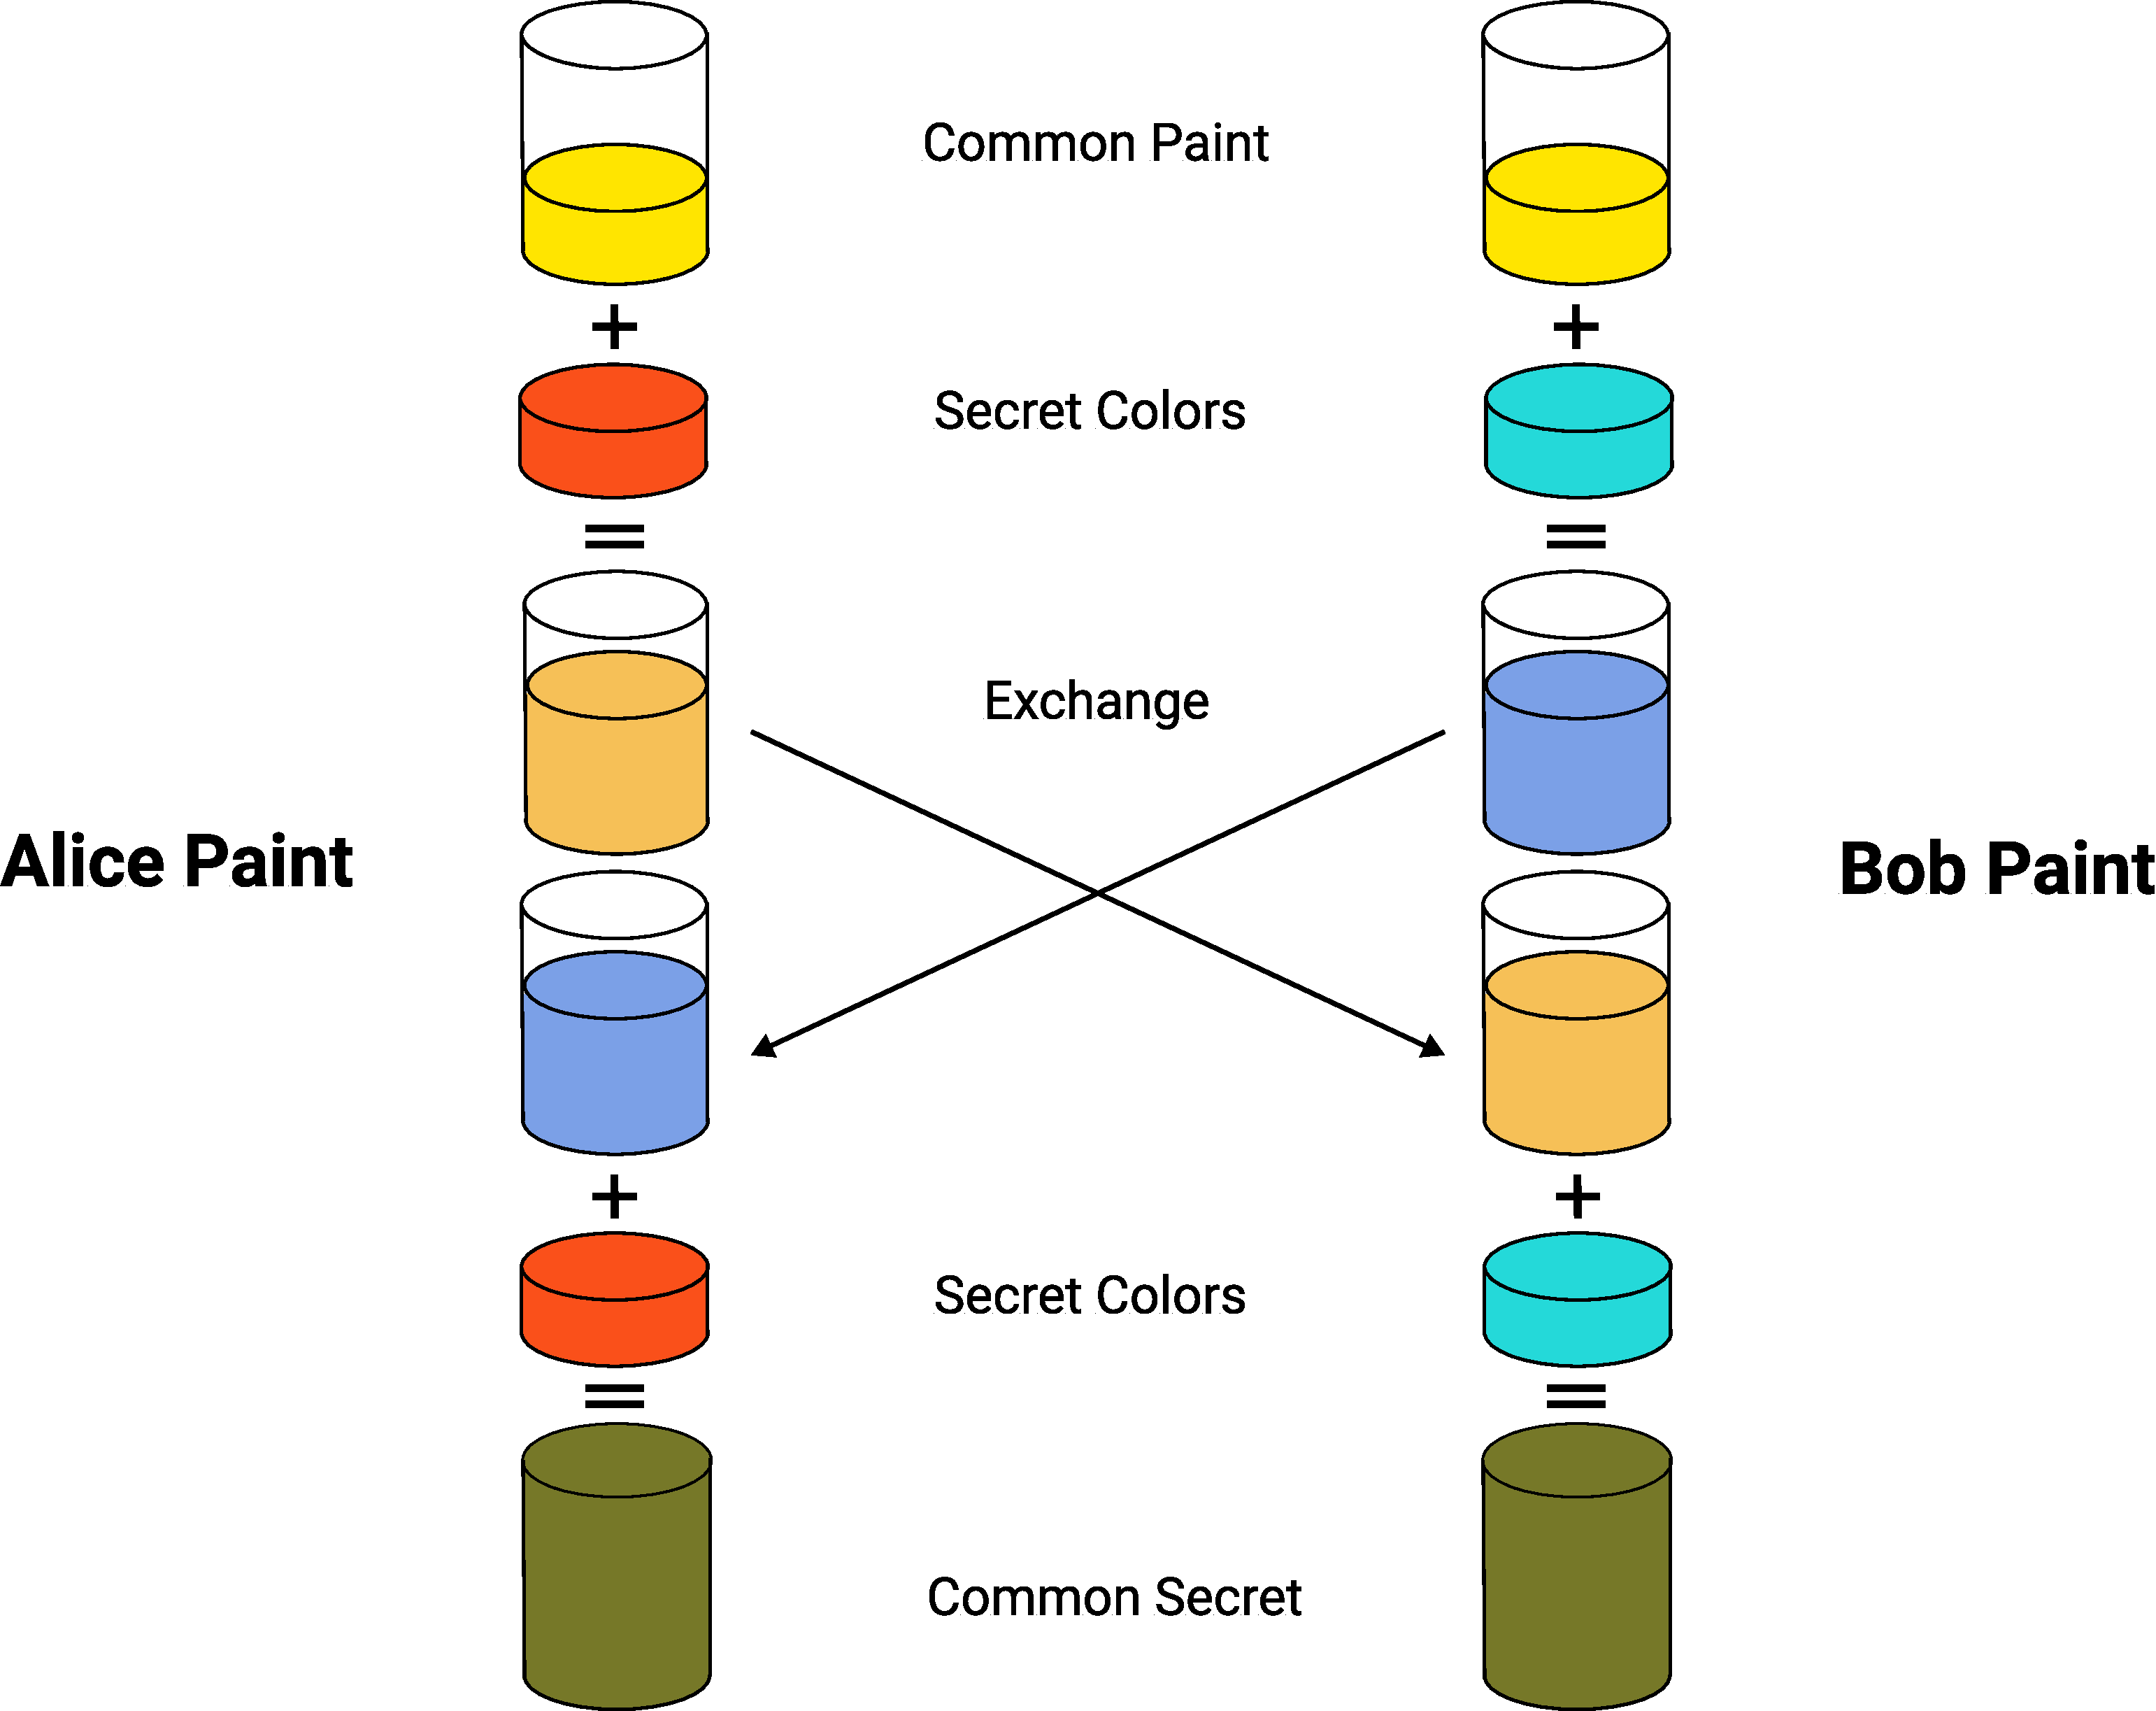
\includegraphics[width=1\textwidth]{Pictures/Diffie-Hellman}
    \caption{Illustration of the concept behind Diffie–Hellman key exchange. Source: }\label{fig:figure4}
\end{figure}
The process begins by having the two parties, Alice and Bob, publicly agree on an arbitrary starting color that does
not need to be kept secret (but should be different every time).
In this example, the color is yellow.
Each person also selects a secret color that they keep to themselves – in this case, red and blue-green.
The crucial part of the process is that Alice and Bob each mix their own secret color together with their mutually
shared color, resulting in orange-tan and light-blue mixtures respectively, and then publicly exchange the two mixed colors.
Finally, each of them mixes the color they received from the partner with their own private color.
The result is a final color mixture (yellow-brown in this case) that is identical to the partner's final color mixture.
If a third party listened to the exchange, it would only know the common color (yellow) and the first mixed colors
(orange-tan and light-blue), but it would be difficult for this party to determine the final secret color (yellow-brown).
Bringing the analogy back to a real-life exchange using large numbers rather than colors, this determination is
computationally expensive.
It is impossible to compute in a practical amount of time even for modern supercomputers.

The simplest and the original implementation of the protocol uses the multiplicative group of integers modulo $P$,
where $P$ is prime, and the generator $G$ which is a primitive root modulo $P$.
These two values are chosen in this way to ensure that the resulting shared secret can take on any value from $1$ to $P-1$.
Here is an example of the protocol
\begin{enumerate}
    \item Given modulus $P$ and generator $G$.
    \item Alice chooses her secret $a$.
    \item Alice sends to Bob $A, \; A = G^a \bmod P$.
    \item Bob chooses his secret $b$.
    \item Bob sends to Alice $B, \; B = G^b \bmod P$.
    \item Alice computes common secret $s, \; s = B^a \bmod P = (G^b \bmod P)^a \bmod P$.
    \item Bob computes common secret $s, \; s = A^b \bmod P = (G^a \bmod P)^b \bmod P$.
    \item Alice and Bob have arrived to the same value
    \[
        A^b \bmod P = G^{ab} \bmod P = G^{ba} \bmod P = B^a \bmod P,
    \]
    more specially,
    \[
        (G^a \bmod P)^b \bmod P = (G^b \bmod P)^a
    \]
\end{enumerate}
However, to reach a satisfactory level of security through DH key exchange a few rules have to be satisfied.
More precisely, Diffie-Hellman works in a multiplicative subgroup of integers modulo a given prime $p$.
To do some DH, you use some DH parameters which are:
\begin{itemize}
    \item p -- a big prime, called the "modulus"
    \item q -- a divisor of $p-1$, called the "subgroup order".
    \item g -- an integer modulo $p$ of order $q$, this means that the smallest integer $k > 0$ such that
    $g^k = 1 \bmod p$ is $k = q$.
\end{itemize}
For DH to be safe, you need the following:

\begin{itemize}
    \item Prime $p$ must defeat attempt at discrete logarithm through Index Calculus.
    This means that $p$ must be large enough, and also must not have any "special structure"
    such as being very close to a power of 2, because such structures allow for improvements in Index Calculus.
    It so happens that size requirements for DH are about the same as the size requirements for RSA,
    though the underlying reason for that is intricate and partly coincidental.
    So, basically, use a random $p$ of 2048 bits, and you will be fine.
    \item Number $q$ should be prime or have a prime divisor whose size is enough to defeat generic algorithms for
    discrete logarithm.
    If the size (in bits) of the largest prime divisor of $q$ is $z$, then generic algorithms have a cost in $2^{z/2}$.
    For best results, arrange for $q$ to be a prime of 256 bits or more.
    \item Systems that use the parameters to perform a DH key exchange must generate a random integer
    between $1$ and $q-1$ uniformly, using a cryptographically strong source of randomness, of course.
    If $q$ is prime and larger than 256 bits, it suffices to choose a 256-bit random value
    to achieve 128-bit of security.
    However, if $q$ is not prime, things are more complex: if $q$ has size $r$ bits,
    and the largest prime divisor of $q$ has size $e$ bits, and $e \geq 256$,
    then one may choose a random value $x$ of size $r-(e-256)$
    bits to get the usual "128-bit security".
    \item When $p$ is a so-called "safe prime", then $p = 2r+1$ for a prime $r$, so for any generator $g$ that is
    not $1$ or $p-1$, the order of $g$ will be either $r$ or $2r$, so it suffices to generate DH secret keys
    $x$ as random 257-bit values.
    The "safe primes" are not actually any safer than other primes,
    except for that point: they tolerate the choice of relatively small DH secret keys for any generator.
    \item Last but not least, DH is a key exchange algorithm that does not,
    inherently, provide authentication or confidentiality.
    DH is "safe" only when used within a protocol that uses DH and other algorithms with proper
    integration to achieve such sought after characteristics as data confidentiality and integrity.
\end{itemize}

Speaking of which, some (many) SSL/TLS implementations did things improperly, in that they
gladly accepted to do DH with weak parameters, in particular a 512-bit modulus.
The protocol itself is suboptimal in its handling of DH because the \texttt{ServerKeyExchange}
message allows the server to send the DH parameters $p$ and $g$ to the client, but not $q$,
leaving the client a bit in the dark.
Thus, the client must either "play safe" and generate its key in the full $1, \;\dots,\; p-1$ range,
or try to use a shorter exponent (say, 256 bits, not 2048) for a reduced computational cost,
but possibly at risk of weakness in case the subgroup order $q$ is not prime.
A better design would have allowed the server to send the value of $q$ and the size of the
biggest prime divisor of $q$.
In that respect, the ECDHE cipher suites of SSL/TLS (DH translated to elliptic curves)
have a better design.

For a practical answer if you are configuring your SSL/TLS server:
you should use a modulus of at least 2048-bit, and a generator $g$ such that the order
of $g$ is a prime $q$ of at least 256 bits;
alternatively, you may use a modulus $p$ which
is a "safe prime", the order of $g$ will then be either a very big prime, or twice
a very big prime, which is almost as good.
Some people feel safer when they generate their DH parameters
"themselves" instead of reusing existing values;
if that's what it takes
to allow you to sleep at night, then do it.

%\subsection{Secrecy Chart}\label{subsec:secrecy-chart}
%The chart below depicts who knows what, again with non-secret values in \textcolor{blue}{blue}, and secret values in \textcolor{red}{red}.
%Here Eve is an eavesdropper – she watches what is sent between Alice and Bob, but she does not alter the contents of their communications.
%\begin{itemize}
%    \item \textcolor{blue}{g} = public (prime) base, known to Alice, Bob, and Eve. $\textcolor{blue}{g = 5}$
%    \item \textcolor{blue}{p} = public (prime) modulus, known to Alice, Bob, and Eve. $\textcolor{blue}{p = 23}$
%    \item \textcolor{red}{a} = Alice's private key, known only to Alice. $\textcolor{red}{a = 6}$
%    \item \textcolor{red}{b} = Bob's private key known only to Bob. $\textcolor{red}{b = 15}$
%    \item \textcolor{blue}{A} = Alice's public key, known to Alice, Bob, and Eve. $\textcolor{blue}{A = g}^{\textcolor{red}{a}} \, mod \, \textcolor{blue}{p = 8}$
%    \item \textcolor{blue}{B} = Bob's public key, known to Alice, Bob, and Eve. $\textcolor{blue}{B = g}^{\textcolor{red}{a}} \, mod \, \textcolor{blue}{p = 8}$
%\end{itemize}
%\begin{center}
%    \begin{table}
%        \begin{tabular}{|c|c|c|c|c|c|}
%            \hline
%            \multicolumn{2}{|c|}{Alice} & \multicolumn{2}{c|}{Bob} & \multicolumn{2}{c|}{Eve}
%            \cr \hline
%            known & unknown & known & unknown & known & unknown
%            \cr \hline
%            $\textcolor{blue}{p = 23}$ & & $\textcolor{blue}{p = 23}$  & & $\textcolor{blue}{p = 23}$ &
%            \cr \hline
%            $\textcolor{blue}{g = 5}$ & & $\textcolor{blue}{g = 5}$ & & $\textcolor{blue}{g = 5}$ &
%            \cr \hline
%            $\textcolor{red}{a = 6}$ & $\textcolor{red}{b}$ & $\textcolor{red}{b = 15}$ & $\textcolor{red}{a}$ & & $\textcolor{red}{a, b}$
%            \cr \hline
%            $\textcolor{blue}{A = 5}^{\textcolor{red}{a}} \, mod \, \textcolor{blue}{23}$ & & $\textcolor{blue}{B = 5}^{\textcolor{red}{b}} \, mod \, \textcolor{blue}{23}$ & & &
%            \cr \hline
%            $\textcolor{blue}{A = 5}^{\textcolor{red}{6}} \, mod \, \textcolor{blue}{23} = \textcolor{blue}{8}$ & & $\textcolor{blue}{B = 5}^{\textcolor{red}{15}} \, mod \, \textcolor{blue}{23} = \textcolor{blue}{19}$ & & &
%            \cr \hline
%            $\textbf{\textcolor{blue}{B}} = \textbf{\textcolor{blue}{19}}$ & & $\textbf{\textcolor{blue}{A}} = \textbf{\textcolor{blue}{8}}$ & & $\textcolor{blue}{A} = \textcolor{blue}{8}$, $\textcolor{blue}{B} = \textcolor{blue}{19}$ &
%            \cr \hline
%            $\textbf{\textcolor{red}{s}} = \textcolor{blue}{B}^{\textcolor{red}{a}} \, mod \, \textcolor{blue}{23}$ & & $\textbf{\textcolor{red}{s}} = \textcolor{blue}{A}^{\textcolor{red}{b}} \, mod \, \textcolor{blue}{23}$ & & &
%            \cr \hline
%            $\textbf{\textcolor{red}{s}} = \textcolor{blue}{19}^{\textcolor{red}{6}} \, mod \, \textcolor{blue}{23} = \textcolor{red}{2}$ & & $\textbf{\textcolor{red}{s}} = \textcolor{blue}{A}^{\textcolor{red}{b}} \, mod \, \textcolor{blue}{23} = \textcolor{red}{2}$ & & &
%            \cr \hline
%
%        \end{tabular}
%        \label{tab:table}
%    \end{table}
%\end{center}
%Now \textcolor{red}{s} is the shared secret key and it is known to both Alice and Bob, but not to Eve.
%Note that it is not helpful for Eve to compute \textcolor{blue}{AB}, which equals
%$\textcolor{blue}{g}^{\textcolor{red}{a} + \textcolor{red}{b}} \, mod \, \textcolor{blue}{p}$.
%Note that it should be difficult for Alice to solve for Bob's private key or for Bob to solve for Alice's private key.
%If it is not difficult for Alice to solve for Bob's private key (or vice versa), Eve may simply substitute her own
%private / public key pair, plug Bob's public key into her private key, produce a fake shared secret key, and solve for
%Bob's private key (and use that to solve for the shared secret key.
%Eve may attempt to choose a public / private key pair that will make it easy for her to solve for Bob's private key).

\begin{figure}[H]
    \centering
    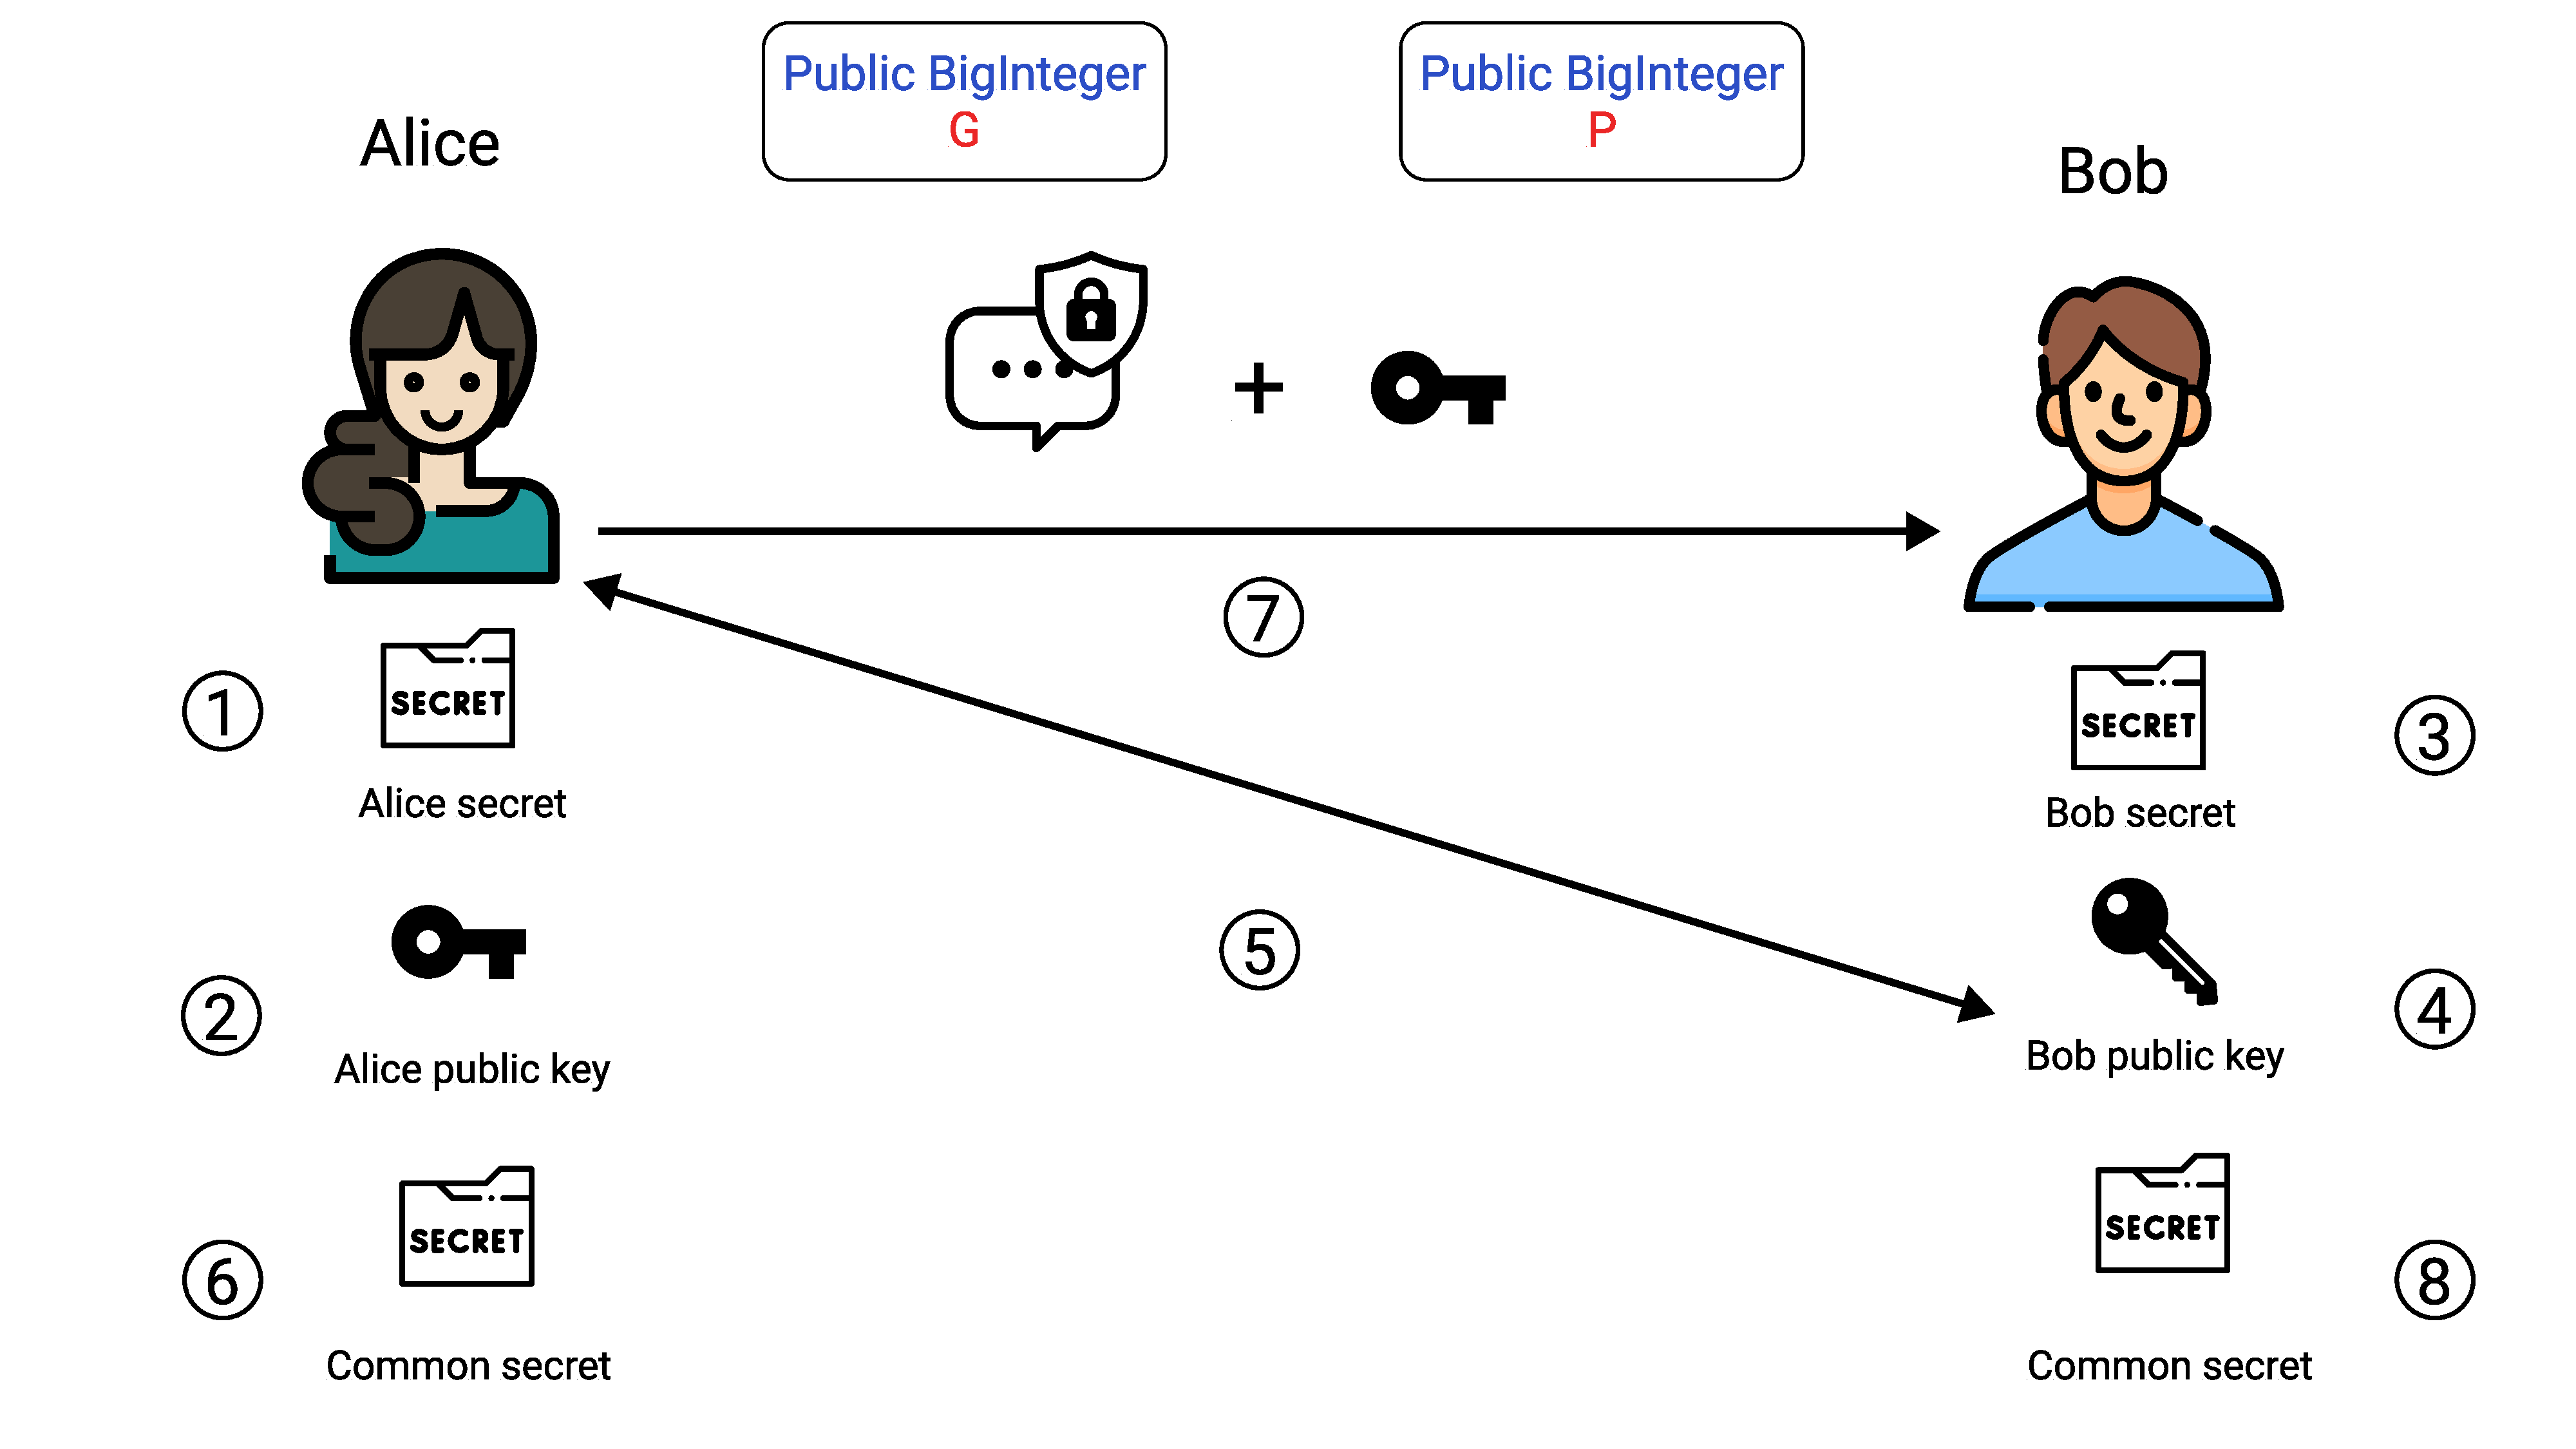
\includegraphics[width=1\textwidth]{Pictures/Key_Exchange}
    \caption{Secret chat encryption concept diagram. Source: }\label{fig:figure7}
\end{figure}
Assume that Alice wants to write a secret message to the Bob.
The secret chat encryption implemented as follows
\begin{enumerate}
    \item Given two public constants: $P, G$.
    \item Alice generates her secret $a$.
    \item Alice generates public key $A$ as $A=G^a \bmod P$ and shares it public.
    \item Bob generates his secret $b$.
    \item Bob generates public key $B$ as $B=G^b \bmod P$ and shares it public.
    \item Alice reads Bob's public key $B$.
    \item Alice calculates Common secret $s$ as $s = B^a \bmod P$.
    \item Alice encrypts message using AES256 algorithm, then sends it to Bob along her public key $A$.
    \item Bob calculates Common secret $s$ as $s = A^b \bmod P$ and decrypts message from Alice.
\end{enumerate}
Although, DH fits the key exchange concerns fine, the secret might be shared via RSA approach as well.
We discuss it in next section.


\section{Planned technologies}\label{sec:planned-technologies}
\begin{itemize}
    \item \textbf{SDK}: \href{https://dotnet.microsoft.com/download/dotnet/5.0}{.NET Core 5.0}
    \item \textbf{Database}
    \begin{itemize}
        \item SQL Database: \href{https://www.postgresql.org/}{PostgreSQL 13}
        \item ORM: \href{https://www.nuget.org/packages/Microsoft.EntityFrameworkCore/5.0.7?_src=template}{Entity Framework Core 5.0.7}
        \item PostgreSQL Provider: \href{https://www.nuget.org/packages/Npgsql.EntityFrameworkCore.PostgreSQL/5.0.7?_src=template}{Npgsql.EntityFrameworkCore.PostgreSQL 5.0.7}
    \end{itemize}
    \item \textbf{Authorization}
    \begin{itemize}
        \item JWT Library: \href{https://www.nuget.org/packages/System.IdentityModel.Tokens.Jwt}{System JWT 6.8.0}
        \item JWT Library: \href{https://www.nuget.org/packages/System.IdentityModel.Tokens}{System Tokens 6.11.1}
        \item JWT Bearer: \href{https://www.nuget.org/packages/Microsoft.AspNetCore.Authentication.JwtBearer/5.0.7?_src=template}{Microsoft Jwt Bearer 5.0.7}
    \end{itemize}
    \item \textbf{Infrastructure}
    \begin{itemize}
        \item Mediator Pattern Library: \href{https://www.nuget.org/packages/MediatR/9.0.0?_src=template}{MediatR 9.0.0}
        \item Validation Library: \href{https://www.nuget.org/packages/FluentValidation/10.2.3?_src=template}{Fluent Validation 10.2.3}
    \end{itemize}
    \item \textbf{Presentation}
    \begin{itemize}
        \item Documentation: \href{https://www.nuget.org/packages/Swashbuckle.AspNetCore/5.6.3?_src=template}{Swashbuckle 6.1.4}
        \item Realtime Communication: \href{https://www.nuget.org/packages/Microsoft.AspNet.SignalR/}{SignalR 2.4.2}
        \item FrontEnd Development: \href{https://angular.io/guide/setup-local}{Angular 11.2.7}
    \end{itemize}
    \item \textbf{Unit and Integration Testing}
    \begin{itemize}
        \item Testing Framework: \href{https://www.nuget.org/packages/NUnit/}{NUnit 3.13.1}
        \item Testing Auxiliary: \href{https://www.nuget.org/packages/Moq/}{Moq 4.16.1}
        \item Testing Auxiliary: \href{https://www.nuget.org/packages/FluentAssertions}{FluentAssertions 6.0.0}
    \end{itemize}
    \item \textbf{Static Code Analysis}: \href{https://www.sonarqube.org/downloads/}{SonarQube 8.9.2 LTS Community Edition}
    \item \textbf{Containerization}: \href{https://docs.docker.com/desktop/windows/install/}{Docker 3.6.0}
    \item \textbf{Continuous Integration}: \href{https://docs.github.com/en/actions}{GitHub Actions}
\end{itemize}